% Options for packages loaded elsewhere
\PassOptionsToPackage{unicode}{hyperref}
\PassOptionsToPackage{hyphens}{url}
%
\documentclass[
]{book}
\usepackage{amsmath,amssymb}
\usepackage{iftex}
\ifPDFTeX
  \usepackage[T1]{fontenc}
  \usepackage[utf8]{inputenc}
  \usepackage{textcomp} % provide euro and other symbols
\else % if luatex or xetex
  \usepackage{unicode-math} % this also loads fontspec
  \defaultfontfeatures{Scale=MatchLowercase}
  \defaultfontfeatures[\rmfamily]{Ligatures=TeX,Scale=1}
\fi
\usepackage{lmodern}
\ifPDFTeX\else
  % xetex/luatex font selection
\fi
% Use upquote if available, for straight quotes in verbatim environments
\IfFileExists{upquote.sty}{\usepackage{upquote}}{}
\IfFileExists{microtype.sty}{% use microtype if available
  \usepackage[]{microtype}
  \UseMicrotypeSet[protrusion]{basicmath} % disable protrusion for tt fonts
}{}
\makeatletter
\@ifundefined{KOMAClassName}{% if non-KOMA class
  \IfFileExists{parskip.sty}{%
    \usepackage{parskip}
  }{% else
    \setlength{\parindent}{0pt}
    \setlength{\parskip}{6pt plus 2pt minus 1pt}}
}{% if KOMA class
  \KOMAoptions{parskip=half}}
\makeatother
\usepackage{xcolor}
\usepackage{color}
\usepackage{fancyvrb}
\newcommand{\VerbBar}{|}
\newcommand{\VERB}{\Verb[commandchars=\\\{\}]}
\DefineVerbatimEnvironment{Highlighting}{Verbatim}{commandchars=\\\{\}}
% Add ',fontsize=\small' for more characters per line
\usepackage{framed}
\definecolor{shadecolor}{RGB}{248,248,248}
\newenvironment{Shaded}{\begin{snugshade}}{\end{snugshade}}
\newcommand{\AlertTok}[1]{\textcolor[rgb]{0.94,0.16,0.16}{#1}}
\newcommand{\AnnotationTok}[1]{\textcolor[rgb]{0.56,0.35,0.01}{\textbf{\textit{#1}}}}
\newcommand{\AttributeTok}[1]{\textcolor[rgb]{0.13,0.29,0.53}{#1}}
\newcommand{\BaseNTok}[1]{\textcolor[rgb]{0.00,0.00,0.81}{#1}}
\newcommand{\BuiltInTok}[1]{#1}
\newcommand{\CharTok}[1]{\textcolor[rgb]{0.31,0.60,0.02}{#1}}
\newcommand{\CommentTok}[1]{\textcolor[rgb]{0.56,0.35,0.01}{\textit{#1}}}
\newcommand{\CommentVarTok}[1]{\textcolor[rgb]{0.56,0.35,0.01}{\textbf{\textit{#1}}}}
\newcommand{\ConstantTok}[1]{\textcolor[rgb]{0.56,0.35,0.01}{#1}}
\newcommand{\ControlFlowTok}[1]{\textcolor[rgb]{0.13,0.29,0.53}{\textbf{#1}}}
\newcommand{\DataTypeTok}[1]{\textcolor[rgb]{0.13,0.29,0.53}{#1}}
\newcommand{\DecValTok}[1]{\textcolor[rgb]{0.00,0.00,0.81}{#1}}
\newcommand{\DocumentationTok}[1]{\textcolor[rgb]{0.56,0.35,0.01}{\textbf{\textit{#1}}}}
\newcommand{\ErrorTok}[1]{\textcolor[rgb]{0.64,0.00,0.00}{\textbf{#1}}}
\newcommand{\ExtensionTok}[1]{#1}
\newcommand{\FloatTok}[1]{\textcolor[rgb]{0.00,0.00,0.81}{#1}}
\newcommand{\FunctionTok}[1]{\textcolor[rgb]{0.13,0.29,0.53}{\textbf{#1}}}
\newcommand{\ImportTok}[1]{#1}
\newcommand{\InformationTok}[1]{\textcolor[rgb]{0.56,0.35,0.01}{\textbf{\textit{#1}}}}
\newcommand{\KeywordTok}[1]{\textcolor[rgb]{0.13,0.29,0.53}{\textbf{#1}}}
\newcommand{\NormalTok}[1]{#1}
\newcommand{\OperatorTok}[1]{\textcolor[rgb]{0.81,0.36,0.00}{\textbf{#1}}}
\newcommand{\OtherTok}[1]{\textcolor[rgb]{0.56,0.35,0.01}{#1}}
\newcommand{\PreprocessorTok}[1]{\textcolor[rgb]{0.56,0.35,0.01}{\textit{#1}}}
\newcommand{\RegionMarkerTok}[1]{#1}
\newcommand{\SpecialCharTok}[1]{\textcolor[rgb]{0.81,0.36,0.00}{\textbf{#1}}}
\newcommand{\SpecialStringTok}[1]{\textcolor[rgb]{0.31,0.60,0.02}{#1}}
\newcommand{\StringTok}[1]{\textcolor[rgb]{0.31,0.60,0.02}{#1}}
\newcommand{\VariableTok}[1]{\textcolor[rgb]{0.00,0.00,0.00}{#1}}
\newcommand{\VerbatimStringTok}[1]{\textcolor[rgb]{0.31,0.60,0.02}{#1}}
\newcommand{\WarningTok}[1]{\textcolor[rgb]{0.56,0.35,0.01}{\textbf{\textit{#1}}}}
\usepackage{longtable,booktabs,array}
\usepackage{calc} % for calculating minipage widths
% Correct order of tables after \paragraph or \subparagraph
\usepackage{etoolbox}
\makeatletter
\patchcmd\longtable{\par}{\if@noskipsec\mbox{}\fi\par}{}{}
\makeatother
% Allow footnotes in longtable head/foot
\IfFileExists{footnotehyper.sty}{\usepackage{footnotehyper}}{\usepackage{footnote}}
\makesavenoteenv{longtable}
\usepackage{graphicx}
\makeatletter
\def\maxwidth{\ifdim\Gin@nat@width>\linewidth\linewidth\else\Gin@nat@width\fi}
\def\maxheight{\ifdim\Gin@nat@height>\textheight\textheight\else\Gin@nat@height\fi}
\makeatother
% Scale images if necessary, so that they will not overflow the page
% margins by default, and it is still possible to overwrite the defaults
% using explicit options in \includegraphics[width, height, ...]{}
\setkeys{Gin}{width=\maxwidth,height=\maxheight,keepaspectratio}
% Set default figure placement to htbp
\makeatletter
\def\fps@figure{htbp}
\makeatother
\setlength{\emergencystretch}{3em} % prevent overfull lines
\providecommand{\tightlist}{%
  \setlength{\itemsep}{0pt}\setlength{\parskip}{0pt}}
\setcounter{secnumdepth}{5}
\usepackage{booktabs}
\ifLuaTeX
  \usepackage{selnolig}  % disable illegal ligatures
\fi
\usepackage[]{natbib}
\bibliographystyle{plainnat}
\IfFileExists{bookmark.sty}{\usepackage{bookmark}}{\usepackage{hyperref}}
\IfFileExists{xurl.sty}{\usepackage{xurl}}{} % add URL line breaks if available
\urlstyle{same}
\hypersetup{
  pdftitle={R Zero - do simples ao complexo},
  pdfauthor={Diogo J. A. Silva},
  hidelinks,
  pdfcreator={LaTeX via pandoc}}

\title{R Zero - do simples ao complexo}
\author{Diogo J. A. Silva}
\date{2024-02-05}

\begin{document}
\maketitle

{
\setcounter{tocdepth}{1}
\tableofcontents
}
\hypertarget{bem-vindos}{%
\chapter{Bem-vindos}\label{bem-vindos}}

R zero foi criado para introduzir e orientar novos usuários acadêmicos do programa R e RStudio do absoluto ZERO. A ideia é fornecer os conceitos essenciais para a utilização do R, guiando o leitor através da linguagem R, introduzindo pílulas de conceitos que irão se complementando ao longo dos capítulos.

Já existem livros muito bons sobre o assunto, mas então por que utilizar esse em específico? Eu acredito que o diferencial desse livro é como ele está organizado. Começando com conceitos básicos, e adicionando complexidade de uma forma fluída e didática. Além da introdução ao R, é mostrado como trabalhar de forma eficiente utilizando projetos reprodutíveis e fáceis de compartilhar. Muitos conceitos serão deixados de lado para focar no que realmente é essencial e assim criando um esqueleto conceitual que pode ser aprimorado com o tempo. Portanto, nesse livro, iniciantes terão uma boa base introdutória no R mostrando de forma prática como trabalhar com seus dados de forma mais simples.

A ideia é que esse seja o primeiro livro de uma coleção de quatro livros que se complementarão:

\begin{itemize}
\tightlist
\item
  R zero: uma introdução ao R
\item
  R zero: manipulação e limpeza de dados
\item
  R zero: análise estatística
\item
  R zero: visualização de dados
\end{itemize}

Juntos esses materiais fornecerão, de forma simples, o arcabouço essencial da ciência de dados acadêmica.

\hypertarget{pruxe9-requisitos}{%
\chapter{Pré-requisitos}\label{pruxe9-requisitos}}

\hypertarget{instalando-r-e-rstudio}{%
\section{Instalando R e RStudio}\label{instalando-r-e-rstudio}}

Para utilizar este livro de maneira otimizada, é necessário ter o \textbf{R} e o \textbf{RStudio} instalados. Não vou abordar a instalação aqui, pois acredito que você é capaz de encontrar tutoriais simples feitos por uma crianca de 8 anos no YouTube.

Brincadeiras à parte, a ideia é facilitar sua vida. Então saiba o seguinte. O R é o programa principal, o RStudio é uma ``skin'', uma ``roupagem'' do R. Alguns chamam essa roupagem de Ambiente de Desenvolvimento Integrado (IDE - Integrated Development Environment), mas você só precisa saber disso por um motivo: você precisa instalar o R primeiro, depois sua skin (o RStudio), caso contrário ocorrerão problemas.

O \textbf{RStudio} requer \textbf{R 3.3.0} ou superior. Clique no link abaixo, acesse o site para baixar o \textbf{R} e escolha uma versão compatível com o sistema operacional do seu computador.

\begin{enumerate}
\def\labelenumi{\arabic{enumi}.}
\tightlist
\item
  Para baixar e instalar o \textbf{R}, acesse:
\end{enumerate}

\url{https://cran.r-project.org/}

\begin{enumerate}
\def\labelenumi{\arabic{enumi}.}
\setcounter{enumi}{1}
\tightlist
\item
  Em seguida, faça o download e instale o \textbf{RStudio} através do link:
\end{enumerate}

\url{https://posit.co/download/rstudio-desktop/\#download}

\hypertarget{r-para-iniciantes}{%
\chapter{R para iniciantes}\label{r-para-iniciantes}}

Caro iniciante, meu objetivo aqui é mostrar que utilizar o R é muito divertido e recompensador. Você vai perceber que cada código rodado (e que funciona) vai te dar um pouquinho de dopamina e uma sensação de prazer. Claro que alguns erros vão te deixar maluco, mas você vai perceber que tudo é culpa sua. Mas não se preocupe, se é culpa sua, você pode consertá-los :)

A tendência é que, quanto mais você utilizar o R, mais fácil sua vida se tornará, e, apesar da curva de aprendizagem ser um pouco desestimuladora, é 1000 vezes recompensadora. Como alguns gostam de dizer, você conseguirá fazer um gráfico até 30 vezes mais rápido! Não sei de onde veio esse cálculo, mas se está na internet, é verdade.

\hypertarget{entendendo-o-rstudio}{%
\section{Entendendo o RStudio}\label{entendendo-o-rstudio}}

Tudo que faremos será através do R Studio devido à organização que ele nos fornece. O RStudio é uma roupagem para o R, que nos oferece um ambiente de trabalho mais amigável e organizado. Se você seguiu as instruções de instalação corretamente, terá dois ícones, o do R base e o do RStudio. Vamos abrir o programa RStudio dando dois cliques sobre seu ícone (Figura 1).

\begin{figure}
\centering

\includegraphics[width=2.08333in,height=\textheight]{img/rstudio_logo.png}
\caption{Figura 1. Icone do RStudio}
\end{figure}

Ao abrir o R Studio, você verá o seguinte:
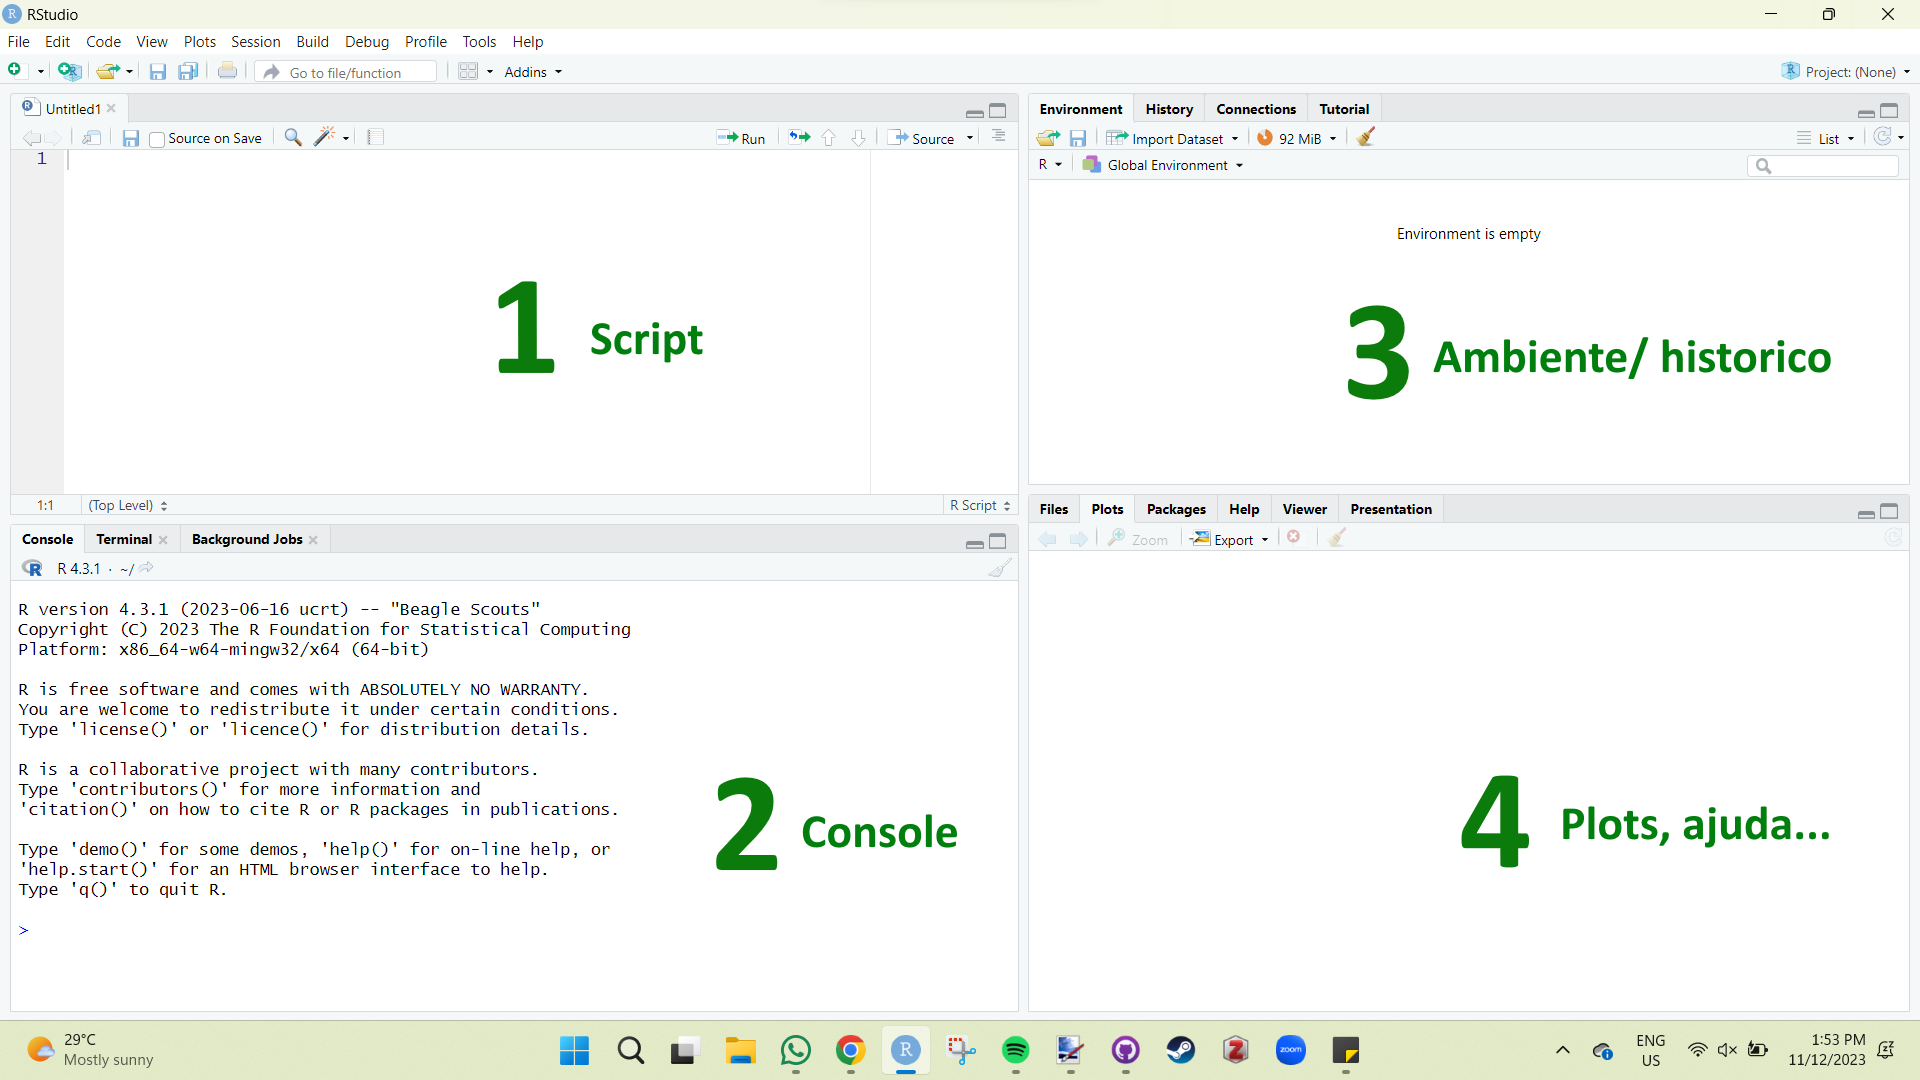
\includegraphics{img/cara_do_rstudio1.png}

Não tem a aparência convencional dos programas estatísticos, mas isso acontece porque não se realizam tarefas clicando em abas ou botões. No R Studio, você executa comandos por meio de códigos! No futuro, é provável que exista um programa com o qual você poderá conversar em qualquer idioma, e ele realizará as tarefas que você pedir. Não, pera, isso já existe! Chama-se inteligência artificial! Entretanto, não se deixe enganar. Os conhecimentos íntimos de como pensar, organizar, analisar e mostrar seus dados são importantíssimos para todo um projeto científico. Mas se isso não te convence, as melhores inteligências artificiais do mercado são pagas e podem te retornar resultados enganosos. Então, tenha muito cuidado e utilize as inteligências artificiais disponíveis apenas como uma ferramenta auxiliar!

Vamos ao que importa: entender como o R funciona. O R possui uma linguagem, e tudo que você vai fazer no R é utilizando essa linguagem, que são verdadeiros comandos. Importe essa planilha! Crie esse gráfico! Faça a média dessa variável! E por aí vai. Então, vamos dar o nosso primeiro comando para o R e falar diretamente com ele. Pediremos que ele some 1 + 1, e para fazer isso iremos digitar 1 + 1 no console (Figura 2 - janela 2) e apertar a tecla ``Enter''.

\begin{Shaded}
\begin{Highlighting}[]
\DecValTok{1}\SpecialCharTok{+}\DecValTok{1}
\end{Highlighting}
\end{Shaded}

\begin{itemize}
\tightlist
\item
  \emph{Dica: Utilize este livro realizando os comandos sugeridos diretamente no R Studio. Sinta-se livre para executar outros comandos similares.}
\end{itemize}

Ao fazer isso, ele vai te retornar o valor 2. Você pode utilizar o R como uma calculadora e realizar as operações básicas normalmente. Agora, vamos pedir para ele subtrair 10 - 5, digitando no console e pressionando Enter. Perceba que não faz diferença se você digitar 10-5, 10 - 5, 10-5, ou até mesmo 10 -5. Mas claro que ao escrever códigos, iremos utilizar a forma que mantém o código mais organizado. Minha sugestão é utilizar 10 - 5.

\begin{Shaded}
\begin{Highlighting}[]
\DecValTok{10} \SpecialCharTok{{-}} \DecValTok{5}
\end{Highlighting}
\end{Shaded}

Agora vamos pedir para ele multiplicar:

\begin{Shaded}
\begin{Highlighting}[]
\DecValTok{5} \SpecialCharTok{*} \DecValTok{5}
\end{Highlighting}
\end{Shaded}

E dividir:

\begin{Shaded}
\begin{Highlighting}[]
\DecValTok{10} \SpecialCharTok{/} \DecValTok{2}
\end{Highlighting}
\end{Shaded}

Você deve ter percebido que cada operação matemática possui seu próprio símbolo. A facilidade de encontrar informações na internet é uma das vantagens do R. Ser gratuito, de código aberto e contar com uma comunidade altamente ativa torna o R singular. Ao longo do livro, você encontrará alguns tópicos nos quais peço que realize pequenas tarefas para compreender o código e desenvolver autonomia.

\begin{itemize}
\tightlist
\item
  \emph{Dica: Pesquise como realizar potenciacao no R e calcule 2 elevado a 2. voce pode utilizar o chatgpt!}
\end{itemize}

Massa! Mas você deve concordar comigo que essa forma de interagir com o R não é muito eficiente. Apesar de mostrar o histórico, se você quiser realizar a primeira operação que fizemos (1 + 1), precisará digitar novamente sempre que quiser fazer algo. Por esse motivo, a janela de script (Figura 2 - janela 1) se torna tão importante.

Vamos criar um script e utilizá-lo em uma situação prática. Mas antes, precisamos aprender mais alguns botões. Veja a figura abaixo:

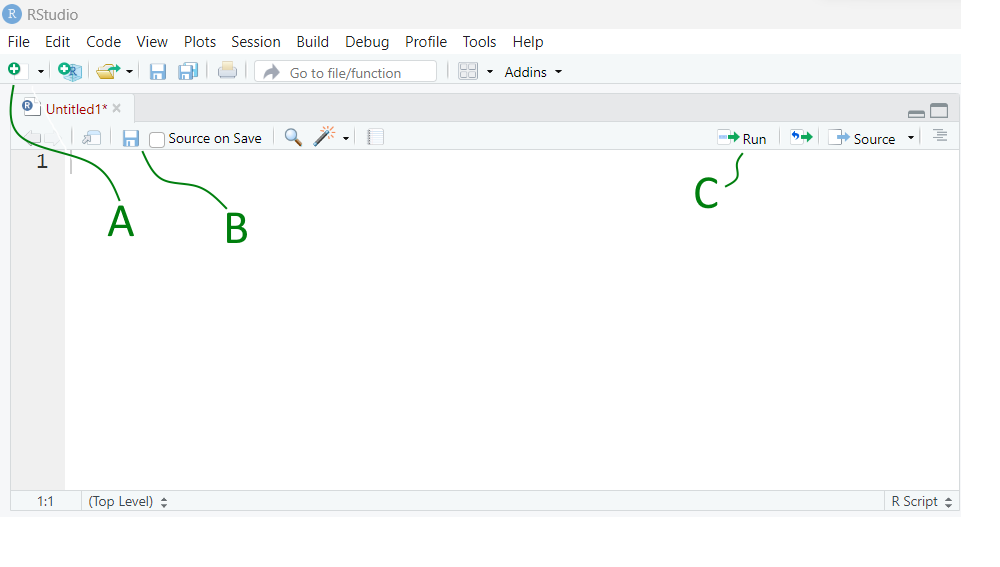
\includegraphics{img/Figura3_script.png}
Vamos criar um novo Script clicando no \textbf{botão ``A'' \textgreater{} New Script}. No Script, podemos digitar livremente sem que o código seja executado; inclusive, podemos fazer comentários utilizando o símbolo \textbf{\#} antes do que foi digitado. Podemos apertar \textbf{Enter} sem enviar o código para o R. O código apenas será executado se clicarmos na linha do código e apertarmos o botão \textbf{``C''} (Run) ou \textbf{Ctrl + Enter}. Copie e cole o código abaixo no seu script e execute, apertando Ctrl + Enter linha por linha. Perceba que o \textbf{\#} impede que o nome Script seja executado. Se você executar Script sem a \#, o R não vai entender e vai dar erro (voce pode tentar fazer isso para ver o que acontece).

\begin{Shaded}
\begin{Highlighting}[]
\CommentTok{\#Script }

\DecValTok{1} \SpecialCharTok{+} \DecValTok{1}
\DecValTok{2}\SpecialCharTok{+} \DecValTok{2}
\DecValTok{10}\SpecialCharTok{/}\DecValTok{2}
\DecValTok{5}\SpecialCharTok{+}\DecValTok{5{-}2}\SpecialCharTok{/}\DecValTok{2}

\CommentTok{\#Fim}
\end{Highlighting}
\end{Shaded}

O comentário também pode ser feito na mesma linha após o código, permitindo utilizar comentários para explicar o que o código faz.

\begin{verbatim}
2*50 #Esse codigo realiza uma multiplicacao.
\end{verbatim}

Por fim, voce pode salvar o Script para acessá-lo sempre que quiser clicando no \textbf{botao ``B''} e selecionando um local no computador. Voce pode acessar esse script salvo sempre que quiser retornar e continuar um trabalho.

\begin{itemize}
\item
  \emph{Dica: Crie um mini script com diferentes funções matematicas do jeito que voce quiser, incluindo comentarios e explicando como realizar isso no R. Use o chatgpt para criar equacoes mais complexas so para ver o poder do R como uma calculadora e como ferramenta auxiliar.}
\item
  \emph{Outra dica: sempre que você estiver no computador e quiser fazer algum cálculo, por mais simples que seja, não use uma calculadora (do PC ou celular), use o R. Praticar é a chave!}
\end{itemize}

\hypertarget{objetos-vetores-e-funuxe7uxf5es}{%
\section{Objetos, vetores e funções}\label{objetos-vetores-e-funuxe7uxf5es}}

\hypertarget{objetos}{%
\subsection{Objetos}\label{objetos}}

Uma das funções mais importantes do R é a capacidade de armazenar valores em objetos. Por exemplo, podemos dizer que o número 1 será atribuído à letra ``\textbf{a}'', e para isso utilizamos o sinal de igual (\textbf{=}). O ``\textbf{a}'' agora é considerado um objeto e aparecerá na janela de Environment (Figura 2 - janela 3).

\begin{Shaded}
\begin{Highlighting}[]
\CommentTok{\# Criando objetos}
\NormalTok{a }\OtherTok{=} \DecValTok{1}  
\NormalTok{b }\OtherTok{=} \DecValTok{2}  
\end{Highlighting}
\end{Shaded}

Entretanto, o sinal de atribuição mais utilizado é a seta (\textbf{\textless-}), devido à sua direcionalidade. Então, vamos adotar esse símbolo de atribuição. Guarde isso na sua cabeça: o código \textbf{\textless-} significa \textbf{atribuir}.

\begin{Shaded}
\begin{Highlighting}[]
\CommentTok{\# Criando Objetos}
\NormalTok{c }\OtherTok{\textless{}{-}} \DecValTok{3} \CommentTok{\# c recebe 3}
\NormalTok{d }\OtherTok{\textless{}{-}} \DecValTok{5} \CommentTok{\# atribuimos 5 ao d}
\end{Highlighting}
\end{Shaded}

Se voce esta copiando e colocando os codigos do livro no seu script, e apertando \textbf{Ctrl + Enter} em cada linha. Voce criou quatro objetos atraves das atribuicoes. Objetos a, b, c, d.~Mas voce so recebera o seu respectivo valor se voce digitar o objeto e executa-lo com Ctrl + Enter.

\begin{Shaded}
\begin{Highlighting}[]
\NormalTok{a}
\NormalTok{b}
\NormalTok{c}
\NormalTok{d}
\end{Highlighting}
\end{Shaded}

Com esses objetos podemos realizar operacoes matematicas.

\begin{Shaded}
\begin{Highlighting}[]
\CommentTok{\#Operacoes com objetos}

\NormalTok{a }\SpecialCharTok{+}\NormalTok{ b}
\NormalTok{c }\SpecialCharTok{*}\NormalTok{ d}
\NormalTok{b}\SpecialCharTok{/}\DecValTok{2}
\DecValTok{2} \SpecialCharTok{*}\NormalTok{ d}

\CommentTok{\#Fim}
\end{Highlighting}
\end{Shaded}

\emph{Nesse momento, meu consagrado aprendiz, eu espero que você esteja realizando diferentes operações matemáticas, utilizando diferentes atribuições}

Podemos atribuir valores em palavras inteiras. Como por exemplo, atribuir 10 ao objeto chamado ``nota'' (ou qualquer outra palavra).

\begin{Shaded}
\begin{Highlighting}[]
\NormalTok{nota }\OtherTok{\textless{}{-}} \DecValTok{10}
\NormalTok{Nota }\OtherTok{\textless{}{-}} \DecValTok{0}
\end{Highlighting}
\end{Shaded}

Perceba que o R detecta as diferenças entre letras maiúsculas (caixa alta) e minúsculas (caixa baixa). Portanto, ``nota'' é diferente de ``Nota''. Muito cuidado com isso. Conheço um rapaz que sempre aparece desesperado dizendo que o código não está funcionando, e 100\% das vezes, é um erro de digitação. Para evitar erros, sugiro sempre utilizar letras minúsculas.

Alguns símbolos não podem ser utilizados para criar objetos, uma vez que são reservados para finalidades internas no R, como por exemplo o `\textbf{-}', ou \textbf{TRUE} / \textbf{FALSE}. Perceba que ao rodar os códigos abaixo, o R irá retornar um erro.

\begin{Shaded}
\begin{Highlighting}[]
\ConstantTok{FALSE} \OtherTok{\textless{}{-}} \DecValTok{2}
\ConstantTok{TRUE} \OtherTok{\textless{}{-}} \DecValTok{5}
\NormalTok{guarda}\SpecialCharTok{{-}}\NormalTok{chuva }\OtherTok{\textless{}{-}} \DecValTok{2}
\end{Highlighting}
\end{Shaded}

Também podemos atribuir uma equação inteira a um objeto. Na verdade, podemos atribuir quase tudo a um objeto: gráficos, resultados, planilhas, etc. Mas isso veremos mais adiante.

\begin{Shaded}
\begin{Highlighting}[]
\CommentTok{\#Note que o underline (\_) funciona bem para separar palavras, assim como ponto (.)}
\NormalTok{guarda\_chuva }\OtherTok{\textless{}{-}} \DecValTok{2}\SpecialCharTok{*}\DecValTok{10}\SpecialCharTok{/}\DecValTok{2}
\NormalTok{guarda\_chuva}

\NormalTok{guarda.roupa }\OtherTok{\textless{}{-}} \DecValTok{2}\SpecialCharTok{*}\DecValTok{100}\SpecialCharTok{/}\DecValTok{10}
\NormalTok{guarda.roupa}
\end{Highlighting}
\end{Shaded}

Alem disso tudo, podemos atribuir um texto a um objeto. Mas para isso o texto precisa estar entre aspas.

\begin{Shaded}
\begin{Highlighting}[]
\CommentTok{\#Atribuindo a palavra "coxinha" ao objeto melhor\_comida}
\NormalTok{melhor\_comida }\OtherTok{\textless{}{-}} \StringTok{"coxinha"}
\NormalTok{melhor\_comida}
\end{Highlighting}
\end{Shaded}

Mas para que serve tudo isso? Por que aprender essas coisas de objetos, atribuições, e sei que lá? A resposta principal é a capacidade de automação e reprodutibilidade das suas análises. Você poderia usar outro programa estatístico? Poderia. Mas confie que o negócio aqui não possui limites.

Vamos criar um exemplo prático para fixar conceitos. Vamos imaginar que queremos calcular quanto gastamos de aluguel por mês e por ano, considerando que pagamos o aluguel semanalmente. Vamos supor que o aluguel por semana seja de 200 reais.

\begin{Shaded}
\begin{Highlighting}[]
\CommentTok{\#Calculando o aluguel}

\NormalTok{aluguel\_semana }\OtherTok{\textless{}{-}} \DecValTok{200}              \CommentTok{\#valor do aluguel por semana (em reais)}
\NormalTok{aluguel\_mes }\OtherTok{\textless{}{-}} \DecValTok{4} \SpecialCharTok{*}\NormalTok{ aluguel\_semana  }\CommentTok{\#considerando que 1 mes possui 4 semanas.}
\NormalTok{aluguel\_ano }\OtherTok{\textless{}{-}} \DecValTok{12} \SpecialCharTok{*}\NormalTok{ aluguel\_mes    }\CommentTok{\#Para o aluguel por ano basta apenas multiplicar o aluguem mes por 12.}

\CommentTok{\#Aqui vemos o resultado de cada um deles (Ctrl + Enter neles)}
\NormalTok{aluguel\_semana}
\NormalTok{aluguel\_mes}
\NormalTok{aluguel\_ano}
\end{Highlighting}
\end{Shaded}

Veja que massa! Criamos um script para calcular o valor do aluguel por mês e por ano. Com esse script, você pode calcular facilmente diferentes situações, simulando diferentes valores de aluguel. Para isso, é só alterar o valor 200 de \textbf{aluguel\_semana} para o valor desejado e rodar linha por linha.

\begin{itemize}
\tightlist
\item
  \emph{Dica: crie o objeto aluguel\_dia que te dara a possibilidade de contabilizar qualquer quantidade de dias, bastando apenas multiplicar o objeto (aluguel\_dia) pela quantidade de dias desejado.}
\end{itemize}

Se você pode fazer isso para calcular o aluguel, imagine o que esse sistema pode fazer pela sua análise de dados.

\hypertarget{vetores}{%
\subsection{Vetores}\label{vetores}}

Os objetos com múltiplos valores do mesmo tipo são chamados de vetores. Para criar um vetor, inserimos os valores dentro de parênteses separados por vírgulas. Vírgulas no R servem para separar o código. Então, se você quiser digitar números quebrados, nunca utilize \textbf{vírgula}, utilize \textbf{ponto}.

\begin{Shaded}
\begin{Highlighting}[]
\NormalTok{vetor.a }\OtherTok{\textless{}{-}} \FunctionTok{c}\NormalTok{(}\DecValTok{2}\NormalTok{, }\DecValTok{8}\NormalTok{, }\DecValTok{15}\NormalTok{)}
\NormalTok{vetor.b }\OtherTok{\textless{}{-}} \FunctionTok{c}\NormalTok{(}\FloatTok{2.5}\NormalTok{, }\FloatTok{2.2}\NormalTok{, }\FloatTok{2.1}\NormalTok{)}
\NormalTok{melhores\_comidas }\OtherTok{\textless{}{-}} \FunctionTok{c}\NormalTok{(}\StringTok{"coxinha"}\NormalTok{,}\StringTok{"pastel"}\NormalTok{,}\StringTok{"lasanha"}\NormalTok{) }\CommentTok{\#Lembre{-}se, caracteres precisam estar dentro de aspas.}

\NormalTok{vetor.a}
\NormalTok{vetor.b}
\NormalTok{Melhores\_comidas}
\end{Highlighting}
\end{Shaded}

Opa, deu um erro, né? Estou marcando o tempo de quanto tempo você demorou para perceber que o nome do objeto é ``melhores\_comidas'' e não ``Melhores\_comidas'' com M maiúsculo. É só pra ficar ligado.

\hypertarget{funuxe7uxf5es}{%
\subsection{Funções}\label{funuxe7uxf5es}}

No R, as funções servem para processar de alguma forma os dados. O R já possui algumas funções nativas, como, por exemplo, para calcular a raiz quadrada de um número. A função possui um nome, geralmente associado ao que ela faz, e argumentos que são o tipo de dado que você precisa inserir nela para ser calculado. Vamos dar uma olhada na função sqrt(). A sigla ``sqrt'' representa ``square root'' em inglês. Primeiro, vamos rodar a função sem argumentos, apenas o \textbf{sqrt()}, e depois inserimos o argumento, que nesse caso, é um número.

\begin{Shaded}
\begin{Highlighting}[]
\CommentTok{\#funcao que calcula raiz quadrada}

\FunctionTok{sqrt}\NormalTok{()}

\FunctionTok{sqrt}\NormalTok{(}\DecValTok{25}\NormalTok{)}
\end{Highlighting}
\end{Shaded}

Note que quando não colocamos (ou erramos) o argumento, o R vai te retornar um erro, geralmente, explicando o problema.

Existem funções dentro do R para todo tipo de coisa! Vamos criar um vetor (conjunto de dados) e fazer alguns cálculos utilizando algumas funções.

\begin{Shaded}
\begin{Highlighting}[]
\CommentTok{\#Notas do terceiro ano A}
\CommentTok{\#Cada um desses numeros representa uma nota de um aluno}
\NormalTok{notas }\OtherTok{\textless{}{-}} \FunctionTok{c}\NormalTok{(}\DecValTok{10}\NormalTok{, }\DecValTok{8}\NormalTok{, }\DecValTok{7}\NormalTok{, }\DecValTok{5}\NormalTok{, }\DecValTok{2}\NormalTok{, }\DecValTok{4}\NormalTok{, }\FloatTok{6.6}\NormalTok{, }\FloatTok{7.9}\NormalTok{, }\FloatTok{8.9}\NormalTok{, }\FloatTok{9.5}\NormalTok{)}

\CommentTok{\#Qual a media da turma?}
\FunctionTok{mean}\NormalTok{(notas)}

\CommentTok{\#Qual a mediana?}
\FunctionTok{median}\NormalTok{(notas)}

\CommentTok{\#Qual o desvio padrao das notas?}
\FunctionTok{sd}\NormalTok{(notas) }\CommentTok{\#sd vem de standard deviation}

\CommentTok{\#Qual a menor e a maior nota?}
\FunctionTok{min}\NormalTok{(notas)}
\FunctionTok{max}\NormalTok{(notas)}

\CommentTok{\#resumo das notas}
\FunctionTok{summary}\NormalTok{(notas)}
\end{Highlighting}
\end{Shaded}

Cada uma dessas funções realiza algum cálculo específico. No caso de summary(), ela realiza o cálculo da média, mediana, máximo, mínimo e quartis, tudo ao mesmo tempo. Talvez em algum momento você não encontre a função que precisa para determinada tarefa; nesse caso, você pode criar sua própria função! Pode criar uma função utilizando outras funções para fazer algo específico para você. Por enquanto, vamos apenas ser usuários de funções e não criadores. Mas se você realmente quer saber como criar uma função, não irei te limitar. Abaixo, você encontra um dos exemplos mais simples de função. Utilize sua criatividade, seus conhecimentos de objetos, funções e vetores para criar alguma função. Mas sinta-se à vontade para pular essa parte, uma vez que ela não é essencial ao uso do R.

\hypertarget{criando-uma-funcao---parte-i-opcional}{%
\subsubsection{Criando uma funcao - parte I (opcional)}\label{criando-uma-funcao---parte-i-opcional}}

Vamos imaginar que voce precise criar uma funcao para somar dois numeros. Uma funcao simples mas que vai nos ajudar a entender a estrutura de uma funcao. Para criar uma funcao utilizamos uma funcao chamada ``\textbf{function()}''. Essa eh uma funcao que possui dois argumentos numericos que chamamos de x e y. A funcao vai pegar esses dois valores e realizar um calculo, que no caso, eh uma soma simples. O resultado da soma sera atribuido a um objeto chamado ``resultado'', e ele sera mostrado atraves da funcao ``print''. Agora que criamos a funcao, vamos utiliza-la para somar dois numeros qualquer.

\begin{Shaded}
\begin{Highlighting}[]
\CommentTok{\#Criando a funcao soma}

\NormalTok{soma }\OtherTok{\textless{}{-}} \ControlFlowTok{function}\NormalTok{(x, y) \{}

\NormalTok{resultado }\OtherTok{\textless{}{-}}\NormalTok{ x }\SpecialCharTok{+}\NormalTok{ y}
\FunctionTok{print}\NormalTok{(resultado)}

\NormalTok{\}}
\end{Highlighting}
\end{Shaded}

Veja que: o nome ``soma'', a gente que criou, poderia ter sido ``add'' ou ``adição''. Os argumentos da função ficam dentro do parênteses; se existir mais de um, são separados por vírgulas. Dentro das chaves, vem todo o processamento que a gente quis que a função realizasse, no caso, apenas uma soma, e que esse resultado seja mostrado para a gente.

Agora vamos usar essa função. Uma vez criada, ela fica armazenada no R e podemos utilizá-la. Para usá-la, só precisamos fornecer dois números para que esses sejam somados.

\begin{Shaded}
\begin{Highlighting}[]
\CommentTok{\#Utilizando a funcao soma}

\FunctionTok{soma}\NormalTok{(}\DecValTok{2}\NormalTok{,}\DecValTok{2}\NormalTok{) }\CommentTok{\#pode colocar qualquer numero}
\end{Highlighting}
\end{Shaded}

Agora, vamos criar uma função para calcular a velocidade média. Para isso, a gente precisa dividir a distância pelo tempo.

\begin{Shaded}
\begin{Highlighting}[]
\CommentTok{\#Criando funcao}
\NormalTok{vm }\OtherTok{\textless{}{-}} \ControlFlowTok{function}\NormalTok{(distancia, tempo) \{}
\NormalTok{  resultado }\OtherTok{\textless{}{-}}\NormalTok{ distancia }\SpecialCharTok{/}\NormalTok{ tempo}
  \FunctionTok{print}\NormalTok{(resultado)}
\NormalTok{\}}

\CommentTok{\#Utilizando funcao vm (velocidade media)}
\CommentTok{\#a distancia percorrida foi 100km}
\CommentTok{\#o tempo gasto foi 2 horas}

\FunctionTok{vm}\NormalTok{(}\DecValTok{100}\NormalTok{, }\DecValTok{2}\NormalTok{) }\CommentTok{\#resultado deve ser interpretado em km por hora.}
\end{Highlighting}
\end{Shaded}

Você deve estar dizendo ``vish que lezeira, já daria pra ter feito direto haha''. Sim, daria, mas a ideia é aprender a criar uma função. Mais para frente voce vai ver o potencial disso.

\hypertarget{tabela-de-dados}{%
\section{Tabela de dados}\label{tabela-de-dados}}

\hypertarget{data-frame}{%
\subsection{Data frame}\label{data-frame}}

DataFrame nada mais é do que uma tabela de dados. Vamos direto ao que interessa e usar a função \emph{data.frame()} para criar uma tabela. Iremos criar as notas de 10 alunos e seus respectivos nomes. Se você ainda estiver na mesma sessão de R, podemos ver que o objeto ``notas'' ainda está salvo na janela 3 (Environment e History) e podemos aproveitá-lo. De qualquer forma, vou recriar ``notas'', caso por algum motivo você TENHA SAÍDO do R, um absurdo, mas acontece.

\begin{Shaded}
\begin{Highlighting}[]
\CommentTok{\#Criando um data frame contendo as notas e os nomes de cada aluno}

\CommentTok{\#Primeiro criamos as notas (cada numero representa a nota de um aluno)}
\NormalTok{notas }\OtherTok{\textless{}{-}} \FunctionTok{c}\NormalTok{(}\DecValTok{10}\NormalTok{, }\DecValTok{8}\NormalTok{, }\DecValTok{7}\NormalTok{, }\DecValTok{5}\NormalTok{, }\DecValTok{2}\NormalTok{, }\DecValTok{4}\NormalTok{, }\FloatTok{6.6}\NormalTok{, }\FloatTok{7.9}\NormalTok{, }\FloatTok{8.9}\NormalTok{, }\FloatTok{9.5}\NormalTok{) }

\CommentTok{\#Segundo criamos os nomes (na ordem das notas)}
\CommentTok{\#Ex: o primeiro valor do objeto nota (10) representara a nota de Marilia que eh o primeiro nome.}

\NormalTok{nomes }\OtherTok{\textless{}{-}} \FunctionTok{c}\NormalTok{(}\StringTok{"Marilia"}\NormalTok{, }\StringTok{"Jonatas"}\NormalTok{, }\StringTok{"Guilherme"}\NormalTok{, }\StringTok{"Thiago"}\NormalTok{, }
\StringTok{"Fifi"}\NormalTok{, }\StringTok{"Brunnin"}\NormalTok{, }\StringTok{"Diego"}\NormalTok{, }\StringTok{"Mazana"}\NormalTok{, }\StringTok{"Bruna"}\NormalTok{, }\StringTok{"Vitoria"}\NormalTok{)}

\CommentTok{\#Terceiro utilizamos a funcao data.frame() para criar a tabela}
\NormalTok{tabela }\OtherTok{\textless{}{-}} \FunctionTok{data.frame}\NormalTok{(nomes, notas)}
\NormalTok{tabela}
\end{Highlighting}
\end{Shaded}

Esse data.frame (tabela) é uma forma muito simplificada das tabelas que iremos importar de nossos dados reais. No entanto, ela nos serve muito bem para entender como funciona uma planilha no R.

A partir de agora, quero que você perceba uma coisa muito importante e leve isso para a vida. Uma planilha organizada deve ser construída da seguinte forma:

-Variáveis são colunas;
-Observações são linhas;
-Cada valor na sua célula.

Com essa formatação de planilha, você consegue fazer quase tudo no R, para manipulação de dados, construção de gráficos e análises estatísticas.

Logo, para você acessar uma variável de uma tabela, usamos o \textbf{\$} da seguinte forma:

\begin{Shaded}
\begin{Highlighting}[]
\CommentTok{\#Acessando uma variavel}

\NormalTok{tabela}\SpecialCharTok{$}\NormalTok{nomes}
\NormalTok{tabela}\SpecialCharTok{$}\NormalTok{notas}
\end{Highlighting}
\end{Shaded}

Perceba que quando você digita \textbf{tabela\$}, pode apertar a tecla TAB para mostrar e selecionar as variáveis de sua tabela. Caso alguma nota esteja errada e você queira corrigi-la, pode utilizar a função \emph{fix()}. Essa função abre uma janela onde você pode clicar e modificar o valor desejado.

\begin{Shaded}
\begin{Highlighting}[]

\FunctionTok{fix}\NormalTok{(tabela)}
\end{Highlighting}
\end{Shaded}

Quase nunca utilizamos a função \emph{fix()} para corrigir os dados, mas é interessante saber que o R pode abrir novas janelas e criar coisas interativas.

Agora, sabendo como acessar as variáveis de uma tabela, você pode utilizar funções para calcular uma variável específica do data frame.

\begin{Shaded}
\begin{Highlighting}[]
\CommentTok{\#Calculando a media da variavel notas da tabela}
\FunctionTok{mean}\NormalTok{(tabela}\SpecialCharTok{$}\NormalTok{notas)}
\end{Highlighting}
\end{Shaded}

Utilize as funções abaixo para calcular mediana, máximo, mínimo:

\begin{itemize}
\tightlist
\item
  median()
\item
  max()
\item
  min()
\item
  summary()
\end{itemize}

\hypertarget{planilha-de-dados-nativa-do-r}{%
\subsection{Planilha de dados nativa do R}\label{planilha-de-dados-nativa-do-r}}

O R possui um banco de dados que nos fornece algumas tabelas de estudo reais, as quais podemos utilizar para treinar nossas habilidades. Para isso, precisamos dizer para o R qual banco de dados queremos invocar utilizando a função \emph{data()}.

\begin{Shaded}
\begin{Highlighting}[]
\CommentTok{\#Importando o banco de dados "iris" do R}
\FunctionTok{data}\NormalTok{(iris)}

\CommentTok{\#Funcoes exploratorias}
\FunctionTok{head}\NormalTok{(iris) }\CommentTok{\#Mostra a parte de cima da planilha }
\FunctionTok{tail}\NormalTok{(iris) }\CommentTok{\#Mostra a parte de baixo}
\FunctionTok{str}\NormalTok{(iris)  }\CommentTok{\#Mostra os tipos das variaveis}
\end{Highlighting}
\end{Shaded}

Veja que ao usarmos a funcao \emph{str()} o R retorna a natureza das variaveis da planilha.

\begin{itemize}
\tightlist
\item
  \emph{num} significa numerica.
\item
  \emph{Factor} significa que eh uma variavel qualitativa com fatores (setosa, versicolor, virginica).
\end{itemize}

Às vezes, a planilha é importada com as variáveis mal formatadas, e isso pode gerar problemas de reconhecimento por parte do R. Nesse caso, é sempre interessante realizar a verificação dos dados utilizando a função \emph{str()} ou outras funções similares. Caso o R não esteja identificando as variáveis corretamente, duas funções muito úteis podem ser utilizadas: \emph{as.numeric()} e \emph{as.factor()}.

\begin{Shaded}
\begin{Highlighting}[]
\FunctionTok{data}\NormalTok{(iris)}

\CommentTok{\#Convertendo variavel para numerica}
\CommentTok{\#a variavel sepal lenght da tabela iris recebe ela mesma transformado em numera}
\NormalTok{iris}\SpecialCharTok{$}\NormalTok{Sepal.Length }\OtherTok{\textless{}{-}} \FunctionTok{as.numeric}\NormalTok{(iris}\SpecialCharTok{$}\NormalTok{Sepal.Length)}

\CommentTok{\#Convertendo variavel para fator}
\NormalTok{iris}\SpecialCharTok{$}\NormalTok{Species }\OtherTok{\textless{}{-}} \FunctionTok{as.factor}\NormalTok{(iris}\SpecialCharTok{$}\NormalTok{Species)}
\end{Highlighting}
\end{Shaded}

Basicamente, você está transformando em numérica a variável Sepal length da planilha iris e atribuindo a ela mesma. Dessa forma, você faz a alteração de forma permanente. A mesma coisa ocorre com \emph{as.factor()}.

Vamos brincar um pouco com a planilha iris. Primeiro, veja que ela está construída de forma organizada (variáveis nas colunas, observações nas linhas, cada célula um valor). Podemos então realizar o \emph{summary()} para saber a média, mediana, máximo e mínimo da largura da pétala (Petal.Width).

\begin{Shaded}
\begin{Highlighting}[]
\FunctionTok{summary}\NormalTok{(iris}\SpecialCharTok{$}\NormalTok{Petal.Width)}
\end{Highlighting}
\end{Shaded}

Porém, note que existem 3 espécies diferentes. A função \emph{summary()} não leva isso em consideração. O ideal seria calcular o \emph{summary()} para cada espécie. Para isso, temos uma função muito legal chamada \emph{tapply()}, onde: o primeiro argumento é a variável numérica, o segundo é a variável com os fatores, e o terceiro argumento é a função que você quer aplicar.

\begin{Shaded}
\begin{Highlighting}[]
\CommentTok{\#Calculando por especie}
\FunctionTok{tapply}\NormalTok{(iris}\SpecialCharTok{$}\NormalTok{Petal.Width, iris}\SpecialCharTok{$}\NormalTok{Species, summary)}
\end{Highlighting}
\end{Shaded}

\hypertarget{importando-sua-planilha}{%
\subsection{Importando sua planilha}\label{importando-sua-planilha}}

No RStudio, podemos importar uma planilha no formato Excel (xlsx) utilizando o botão na janela Environment (canto superior direito):

\emph{Environment \textgreater{} Import Dataset \textgreater{} From Excel}

Acho pouco eficiente ensinar a importar dados de um diretório. Acho pouco prático, uma vez que temos o botão de importar. Ao invés disso, irei treiná-lo a utilizar projetos de R reprodutíveis e organizados. Ao trabalhar no R, você seguirá um protocolo básico de como tratar os dados a serem analisados. Ao longo do tempo, você será capaz de otimizar esse protocolo e aplicá-lo para quase todo tipo de dado que você possuir. De qualquer forma, saiba que o R trabalha com uma pasta específica chamada de diretório, e para saber qual é o seu diretório padrão, utilize a função \emph{getwd()}:

\begin{Shaded}
\begin{Highlighting}[]
\FunctionTok{getwd}\NormalTok{()}
\end{Highlighting}
\end{Shaded}

Ao executar essa função, o R te retornará o caminho da pasta do diretório padrão atual, que provavelmente é a pasta ``Documentos'' do seu computador.

Para baixar uma planilha de dados fictícios, clique no link abaixo e tente importá-la através do botão \textbf{Import from Excel}.

\href{data/fake_data.xlsx}{Clique aqui para baixar a planilha ficticia}

\hypertarget{graficos}{%
\section{Graficos}\label{graficos}}

Agora começa a parte divertida! A visualização de dados no R tem um potencial quase infinito devido à sua grande capacidade de personalizar cada pedacinho da figura.

\hypertarget{grafico-de-histograma}{%
\subsection{Grafico de histograma}\label{grafico-de-histograma}}

Esse gráfico nos mostra a frequência dos valores da variável de interesse, como por exemplo, o comprimento da pétala das flores do banco de dados iris.

\begin{Shaded}
\begin{Highlighting}[]
\CommentTok{\#Importando banco de dados "iris"}
\FunctionTok{data}\NormalTok{(iris)}

\CommentTok{\#Criando histograma}
\FunctionTok{hist}\NormalTok{(iris}\SpecialCharTok{$}\NormalTok{Sepal.Length)}
\end{Highlighting}
\end{Shaded}

\begin{figure}
\centering
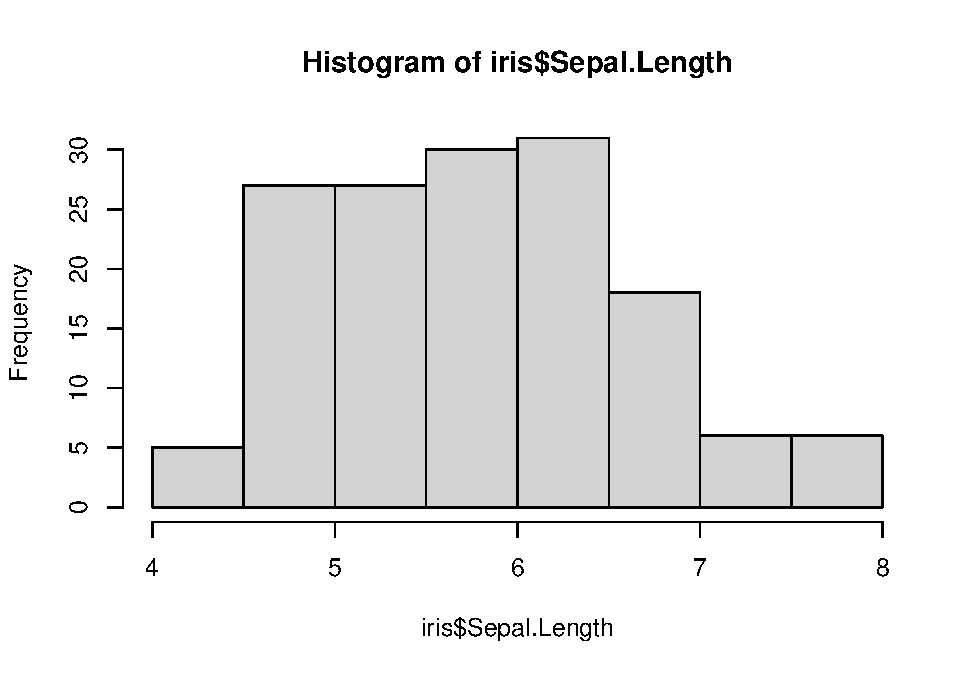
\includegraphics{_main_files/figure-latex/nome-do-chunk1-1.pdf}
\caption{\label{fig:nome-do-chunk1}Gráficos com R base}
\end{figure}

Simples, não é? Mas podemos modificar ainda mais nosso gráfico. Alterar cores, nomes dos eixos, título, etc. Vamos ver mais argumentos com o gráfico de dispersão de pontos.

\hypertarget{grafico-de-dispersao}{%
\subsection{Grafico de dispersao}\label{grafico-de-dispersao}}

Esse gráfico nos mostra a relação entre duas variáveis contínuas. Vamos utilizar o banco de dados ``iris'' para construir e visualizar alguns gráficos. Para construir um gráfico de dispersão, utilizamos a função \emph{plot()}. Note que a função plot possui vários argumentos que podemos ir adicionando para personalizar o gráfico. Além disso, para deixar o código mais organizado, sempre após a vírgula de um argumento, pulamos a linha, de forma que cada argumento fique numa linha.

\begin{Shaded}
\begin{Highlighting}[]
\CommentTok{\#Cria o grafico basico}
\FunctionTok{plot}\NormalTok{(iris}\SpecialCharTok{$}\NormalTok{Sepal.Width, iris}\SpecialCharTok{$}\NormalTok{Petal.Width)}
\end{Highlighting}
\end{Shaded}

\begin{figure}
\centering
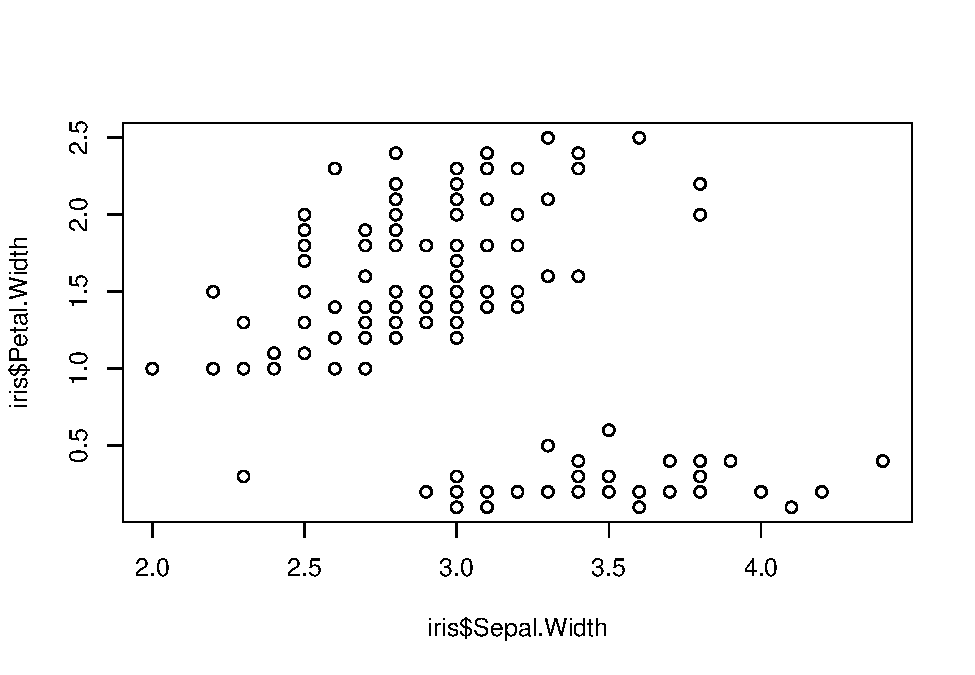
\includegraphics{_main_files/figure-latex/nome-do-chunk2-1.pdf}
\caption{\label{fig:nome-do-chunk2-1}Gráficos com R base}
\end{figure}

\begin{Shaded}
\begin{Highlighting}[]
\CommentTok{\#adiciona o argumento para mudar o nome do eixo y}
\FunctionTok{plot}\NormalTok{(iris}\SpecialCharTok{$}\NormalTok{Sepal.Width, iris}\SpecialCharTok{$}\NormalTok{Petal.Width, }
     \AttributeTok{ylab =} \StringTok{"Petal Width"}\NormalTok{)}
\end{Highlighting}
\end{Shaded}

\begin{figure}
\centering
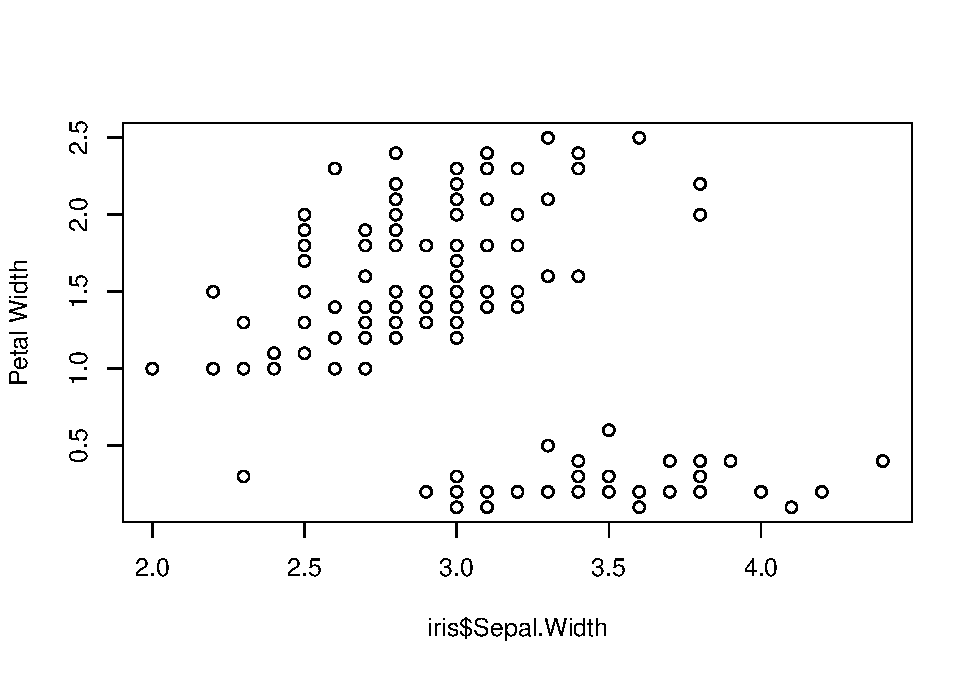
\includegraphics{_main_files/figure-latex/nome-do-chunk2-2.pdf}
\caption{\label{fig:nome-do-chunk2-2}Gráficos com R base}
\end{figure}

\begin{Shaded}
\begin{Highlighting}[]
\CommentTok{\#adiciona o argumento para mudar o nome do eixo x}
\FunctionTok{plot}\NormalTok{(iris}\SpecialCharTok{$}\NormalTok{Sepal.Width, iris}\SpecialCharTok{$}\NormalTok{Petal.Width, }
     \AttributeTok{ylab =} \StringTok{"Petal Width"}\NormalTok{, }
     \AttributeTok{xlab =} \StringTok{"Sepal Width"}
\NormalTok{     )}
\end{Highlighting}
\end{Shaded}

\begin{figure}
\centering
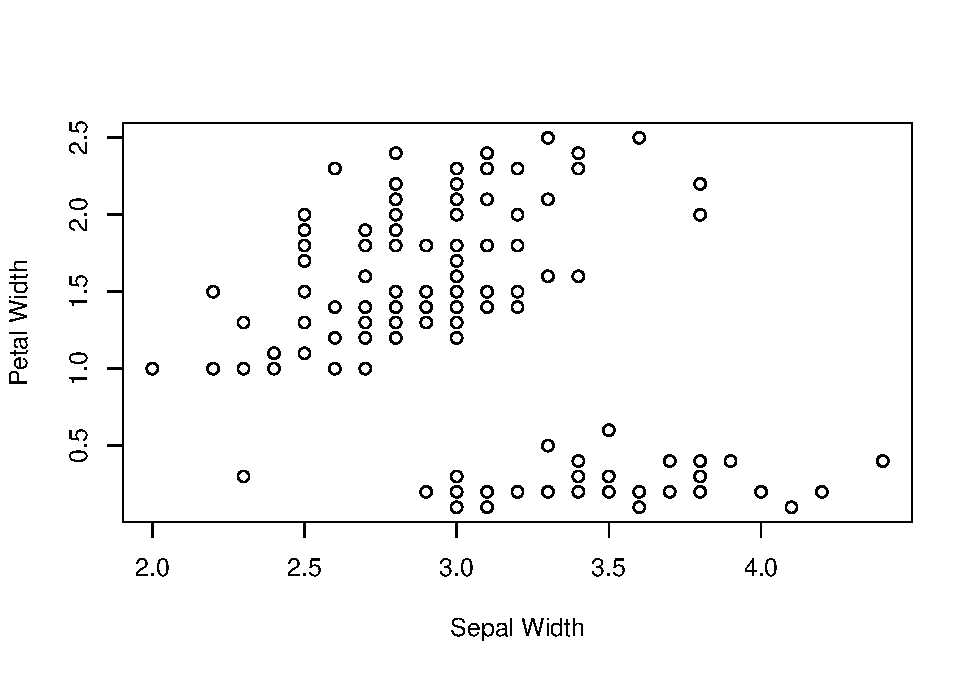
\includegraphics{_main_files/figure-latex/nome-do-chunk2-3.pdf}
\caption{\label{fig:nome-do-chunk2-3}Gráficos com R base}
\end{figure}

\begin{Shaded}
\begin{Highlighting}[]
\CommentTok{\#argumento para mudar a cor dos pontos}
\FunctionTok{plot}\NormalTok{(iris}\SpecialCharTok{$}\NormalTok{Sepal.Width, iris}\SpecialCharTok{$}\NormalTok{Petal.Width, }
     \AttributeTok{ylab =} \StringTok{"Petal Width"}\NormalTok{, }
     \AttributeTok{xlab =} \StringTok{"Sepal Width"}\NormalTok{,}
     \AttributeTok{col =} \StringTok{"blue"}
\NormalTok{     )}
\end{Highlighting}
\end{Shaded}

\begin{figure}
\centering
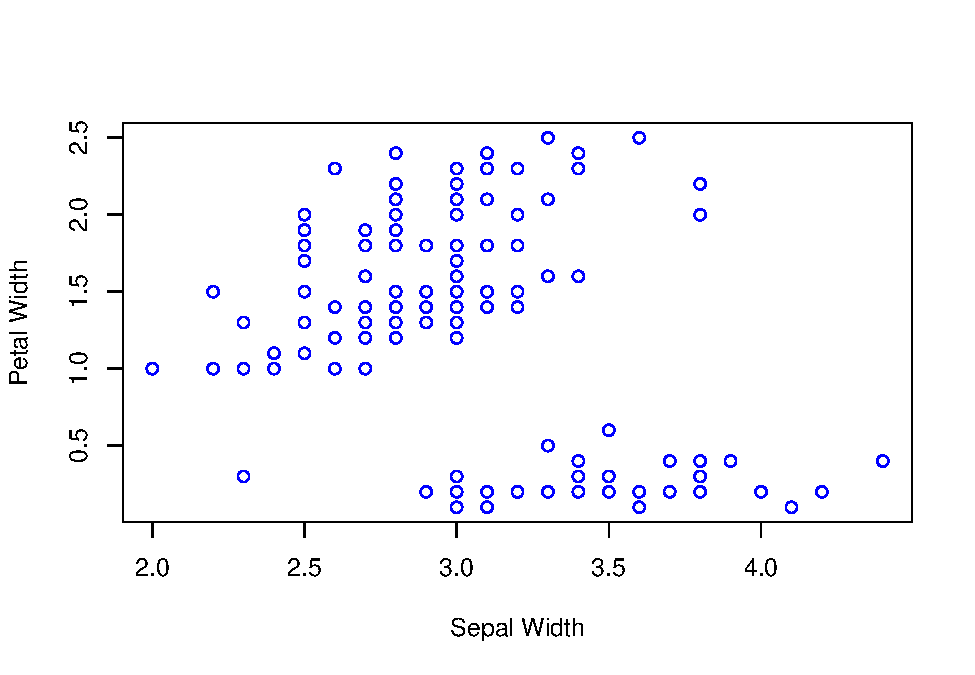
\includegraphics{_main_files/figure-latex/nome-do-chunk2-4.pdf}
\caption{\label{fig:nome-do-chunk2-4}Gráficos com R base}
\end{figure}

\begin{Shaded}
\begin{Highlighting}[]
\CommentTok{\#argumento para mudar o formato dos pontos}
\FunctionTok{plot}\NormalTok{(iris}\SpecialCharTok{$}\NormalTok{Sepal.Width, iris}\SpecialCharTok{$}\NormalTok{Petal.Width, }
     \AttributeTok{ylab =} \StringTok{"Petal Width"}\NormalTok{, }
     \AttributeTok{xlab =} \StringTok{"Sepal Width"}\NormalTok{,}
     \AttributeTok{col =} \DecValTok{3}\NormalTok{,}
     \AttributeTok{pch =} \DecValTok{2}
\NormalTok{     )}
\end{Highlighting}
\end{Shaded}

\begin{figure}
\centering
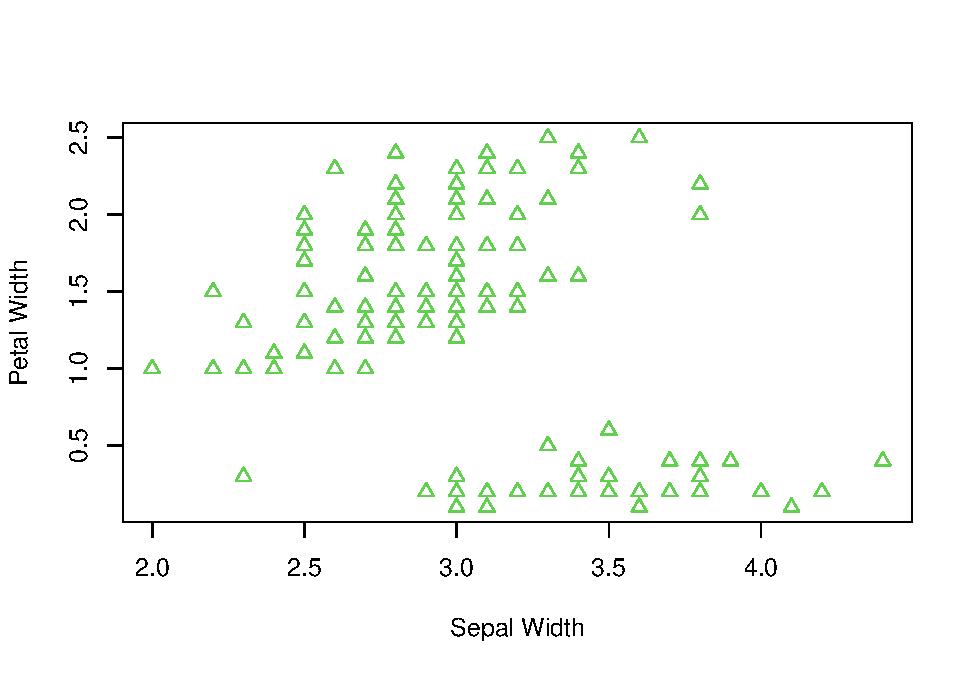
\includegraphics{_main_files/figure-latex/nome-do-chunk2-5.pdf}
\caption{\label{fig:nome-do-chunk2-5}Gráficos com R base}
\end{figure}

\begin{Shaded}
\begin{Highlighting}[]
\CommentTok{\#argumento para adicionar um titulo no grafico}
\FunctionTok{plot}\NormalTok{(iris}\SpecialCharTok{$}\NormalTok{Sepal.Width, iris}\SpecialCharTok{$}\NormalTok{Petal.Width, }
     \AttributeTok{ylab =} \StringTok{"Petal Width"}\NormalTok{, }
     \AttributeTok{xlab =} \StringTok{"Sepal Width"}\NormalTok{,}
     \AttributeTok{col =} \DecValTok{3}\NormalTok{,}
     \AttributeTok{pch =} \DecValTok{2}\NormalTok{,}
     \AttributeTok{main =} \StringTok{"Titulo do grafico"}
\NormalTok{     )}
\end{Highlighting}
\end{Shaded}

\begin{figure}
\centering
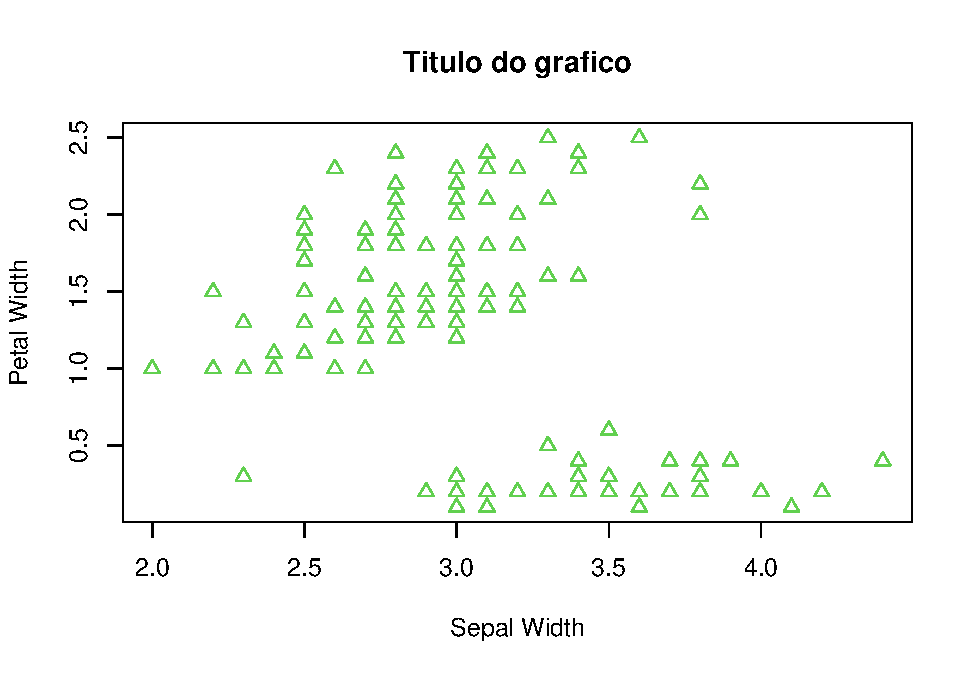
\includegraphics{_main_files/figure-latex/nome-do-chunk2-6.pdf}
\caption{\label{fig:nome-do-chunk2-6}Gráficos com R base}
\end{figure}

\hypertarget{grafico-boxplot}{%
\subsection{Grafico boxplot}\label{grafico-boxplot}}

Para criar o gráfico de boxplot, iremos utilizar a variável numérica Sepal.Width do banco de dados iris em relação à variável Species. Note que na função plot, as duas variáveis (argumentos) eram separadas por vírgula; aqui utilizamos o \textbf{\textasciitilde{}} para relacionar a variável numérica com a categórica.

\begin{Shaded}
\begin{Highlighting}[]
\CommentTok{\#Importa o banco de dados iris}
\FunctionTok{data}\NormalTok{(iris)}

\CommentTok{\#Cria o grafico de boxplot basico}
\FunctionTok{boxplot}\NormalTok{(iris}\SpecialCharTok{$}\NormalTok{Sepal.Width }\SpecialCharTok{\textasciitilde{}}\NormalTok{ iris}\SpecialCharTok{$}\NormalTok{Species)}
\end{Highlighting}
\end{Shaded}

\begin{figure}
\centering
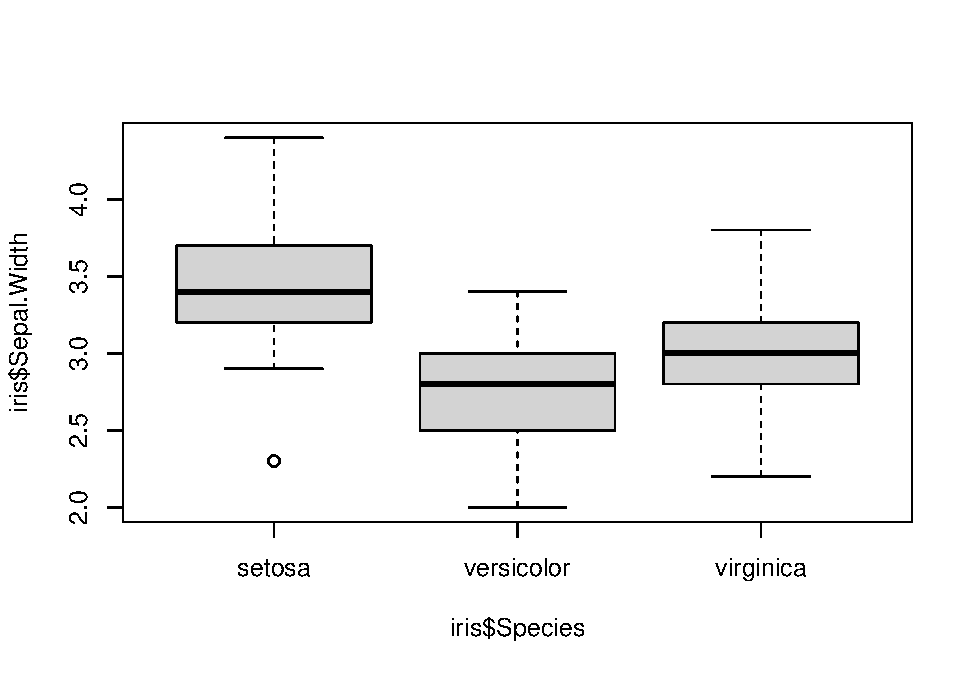
\includegraphics{_main_files/figure-latex/3_basic_boxplot-1.pdf}
\caption{(\#fig:3\_basic\_boxplot-1)Boxplot com R base utilizando o banco de dados iris}
\end{figure}

\begin{Shaded}
\begin{Highlighting}[]
\CommentTok{\#Boxplot personalizado}
\FunctionTok{boxplot}\NormalTok{(iris}\SpecialCharTok{$}\NormalTok{Sepal.Width }\SpecialCharTok{\textasciitilde{}}\NormalTok{ iris}\SpecialCharTok{$}\NormalTok{Species,}
      \AttributeTok{ylab =} \StringTok{"Petal Width"}\NormalTok{, }
      \AttributeTok{xlab =} \StringTok{"Species"}\NormalTok{,}
      \AttributeTok{col =} \FunctionTok{c}\NormalTok{(}\DecValTok{3}\NormalTok{,}\DecValTok{4}\NormalTok{,}\StringTok{"tomato"}\NormalTok{),}
      \AttributeTok{main =} \StringTok{"Titulo do grafico"}
\NormalTok{      )}
\end{Highlighting}
\end{Shaded}

\begin{figure}
\centering
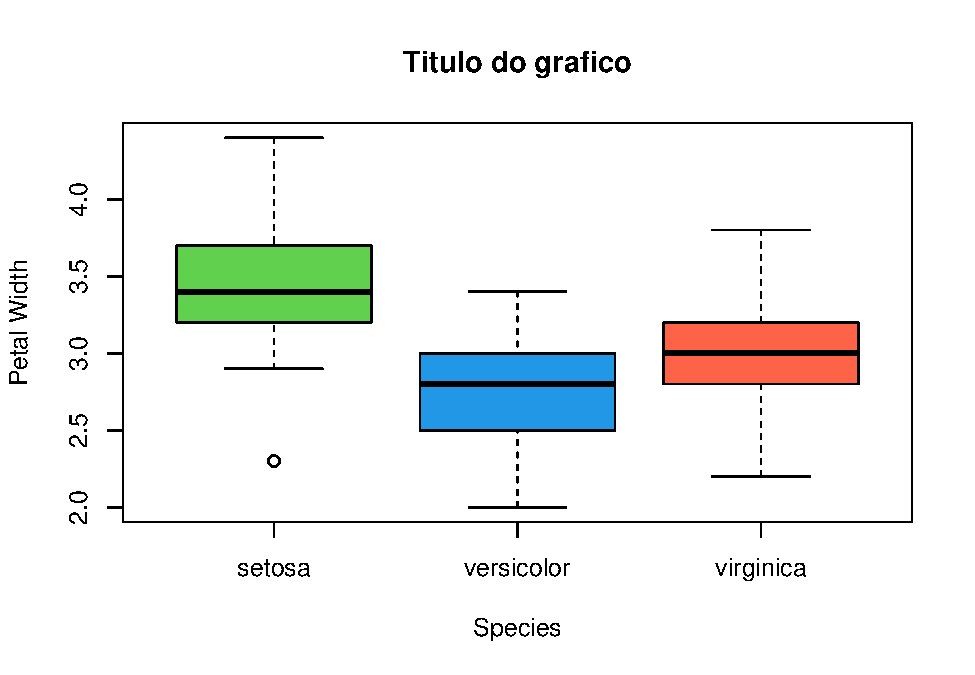
\includegraphics{_main_files/figure-latex/3_basic_boxplot-2.pdf}
\caption{(\#fig:3\_basic\_boxplot-2)Boxplot com R base utilizando o banco de dados iris}
\end{figure}

Perceba que o argumento \textbf{col} pode ser um vetor e pode receber mais de um valor. Nesse caso, demos uma cor para cada fator de Species. Tente substituir os números por outros ou colocar o nome das principais cores como: red, green, blue, yellow\ldots{} Só não esqueça de colocar entre aspas.

\hypertarget{grafico-de-barras}{%
\subsection{Grafico de barras}\label{grafico-de-barras}}

Para criar um gráfico de barras de contagem, vamos criar nosso próprio data frame. Imagine que queremos tabular a contagem total de ectoparasitas (piolho) de aves em cada parte corporal. Como é algo simples, podemos criar diretamente no R.

\begin{Shaded}
\begin{Highlighting}[]
\CommentTok{\#Criando quantidade total de parasitas}
\NormalTok{qt\_parasita }\OtherTok{\textless{}{-}} \FunctionTok{c}\NormalTok{(}\DecValTok{10}\NormalTok{, }\DecValTok{15}\NormalTok{, }\DecValTok{29}\NormalTok{, }\DecValTok{4}\NormalTok{)}

\CommentTok{\#Criando parte corporal da ave}
\NormalTok{parte\_corporal }\OtherTok{\textless{}{-}} \FunctionTok{c}\NormalTok{(}\StringTok{"cabeca"}\NormalTok{, }\StringTok{"asa"}\NormalTok{, }\StringTok{"barriga"}\NormalTok{, }\StringTok{"cauda"}\NormalTok{)}

\CommentTok{\#Criando tabela}
\NormalTok{dados\_parasita }\OtherTok{\textless{}{-}} \FunctionTok{data.frame}\NormalTok{(qt\_parasita, parte\_corporal)}

\CommentTok{\# Cria ndo gráfico de barras}
\NormalTok{grafico }\OtherTok{\textless{}{-}} \FunctionTok{barplot}\NormalTok{(dados\_parasita}\SpecialCharTok{$}\NormalTok{qt\_parasita, }
                   \AttributeTok{names.arg =}\NormalTok{ dados\_parasita}\SpecialCharTok{$}\NormalTok{parte\_corporal,}
                   \AttributeTok{xlab =} \StringTok{"Parte do Corpo"}\NormalTok{,}
                   \AttributeTok{ylab =} \StringTok{"Quantidade de Parasitas"}\NormalTok{,}
                   \AttributeTok{ylim =} \FunctionTok{c}\NormalTok{(}\DecValTok{0}\NormalTok{,}\DecValTok{35}\NormalTok{), }\CommentTok{\#define o limite do eixo y (de 0 a 35)}
                   \AttributeTok{col =} \StringTok{"lightgreen"}\NormalTok{,}
                   \AttributeTok{border =} \StringTok{"black"}\NormalTok{)}

\CommentTok{\# Adicionando os números acima das barras}
\FunctionTok{text}\NormalTok{(grafico, dados\_parasita}\SpecialCharTok{$}\NormalTok{qt\_parasita, }
\AttributeTok{labels =}\NormalTok{ dados\_parasita}\SpecialCharTok{$}\NormalTok{qt\_parasita, }\AttributeTok{pos =} \DecValTok{3}\NormalTok{, }\AttributeTok{cex =} \FloatTok{0.8}\NormalTok{)}
\end{Highlighting}
\end{Shaded}

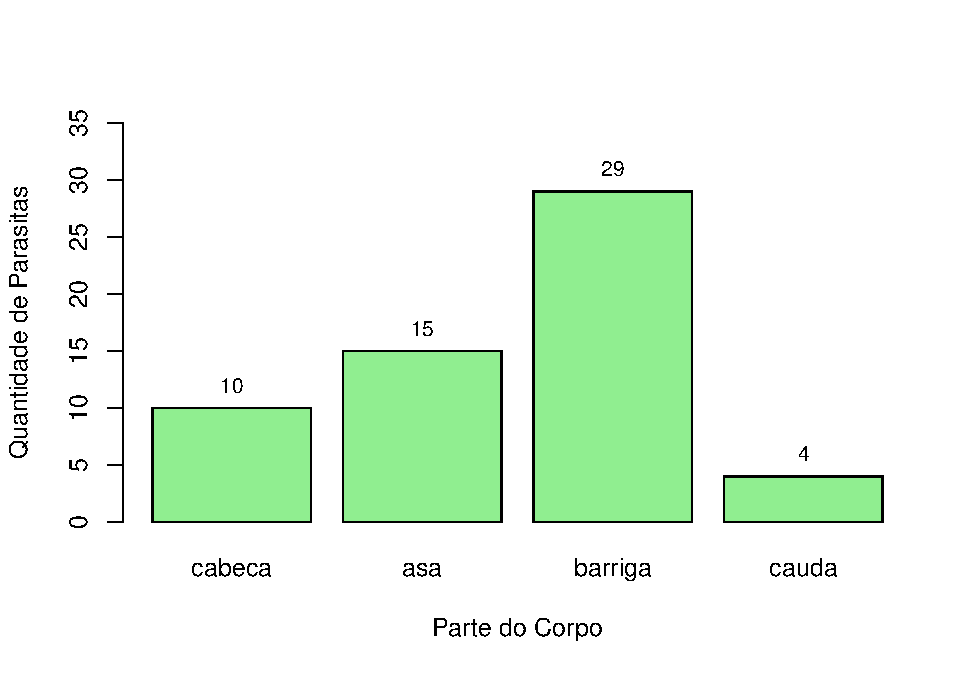
\includegraphics{_main_files/figure-latex/4_basic_hist-1.pdf}
Faça as seguintes modificações no código e veja o que acontece:

\begin{itemize}
\tightlist
\item
  Veja o que acontece se você deletar a linha completa do argumento names.arg.
\item
  Troque o valor 35 de ylim por 50.
\item
  No argumento border, troque ``black'' por ``red'' e depois ``white''.
\item
  Na função text(), troque pos = 3 por pos = 1.
  (rode o gráfico antes para não sobrepor os números)
\end{itemize}

É possível fazer muitos outros tipos de gráficos, utilizando diferentes funções. Mas a ideia desse capítulo é ensinar a utilizar o R, e não a criar gráficos. Então vamos com calma, pois quando você pensar que não, já foi.

\hypertarget{pacotes}{%
\section{Pacotes}\label{pacotes}}

Agora já podemos começar a expandir nosso universo do R. Tudo que fizemos até agora foi utilizando o próprio R base. A partir de agora, iremos incluir um conjunto de novas funções através dos pacotes de R.
Antes de tudo, precisamos instalar o pacote que queremos utilizar, e para isso existem duas formas:

\begin{itemize}
\tightlist
\item
  Utilizando o botão \emph{Tools} do RStudio.
\item
  Utilizando a função \emph{install.packages(``nome\_do\_pacote'')}
\end{itemize}

Vamos instalar o pacote ``lattice'' para criarmos uns gráficos diferentes do que fizemos anteriormente.

Utilizando o botão \emph{Tools} do RStudio clique em: \textbf{Tools \textgreater{} Install package \textgreater{} digite o nome ``lattice''.} Ao começar a digitar, o R irá sugerir opções de pacotes com as iniciais que você digitou. Depois, clique em ``instalar''.

Utilizando a função \emph{install.packages()}

\begin{Shaded}
\begin{Highlighting}[]
\FunctionTok{install.packages}\NormalTok{(}\StringTok{"lattice"}\NormalTok{)}
\end{Highlighting}
\end{Shaded}

O processo de instalação mostra no console vários processos, e enquanto isso acontece, um ícone de ``stop'' vermelho aparece na parte superior direita da janela do console. O processo só termina quando esse ícone some e um aviso aparece:

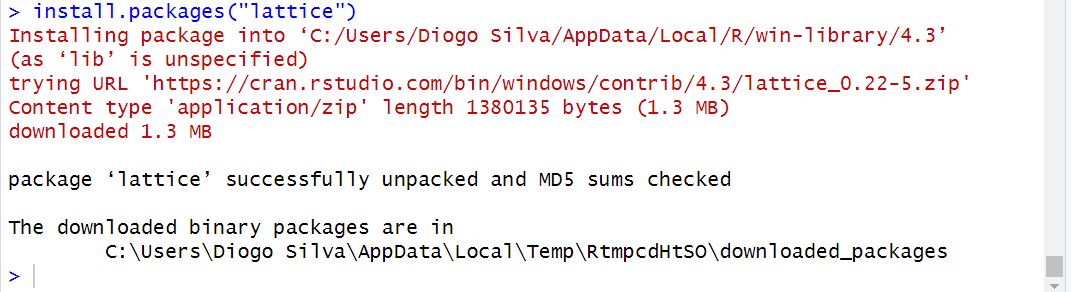
\includegraphics{img/install_package.png}

Pacote instalado, agora é só dizer que queremos utilizar o pacote. O processo de instalação em um determinado computador só precisa ser feito uma vez. Porém, toda vez, você precisa dizer para o R qual pacote você está utilizando. Para isso, utilizamos a função \emph{library()}.

\begin{Shaded}
\begin{Highlighting}[]
\CommentTok{\#Carregando o pacote lattice}
\FunctionTok{library}\NormalTok{(lattice)}
\end{Highlighting}
\end{Shaded}

Se você carregou o pacote e o R não te retornou nenhum erro, está tudo certo. Às vezes, ele te retorna um Warning message, também está tudo certo. Vamos adiante.

O pacote lattice que acabamos de instalar nos fornece várias funções para criação de gráficos. Tenha em mente que existem milhares de pacotes, cada um trazendo um conjunto de funções e bancos de dados de diferentes contextos, tanto para criar gráficos quanto para realizar modelos estatísticos avançados.

Vamos criar alguns gráficos utilizando as funções que o pacote lattice nos forneceu.

\begin{Shaded}
\begin{Highlighting}[]
\CommentTok{\#Se o pacote já estiver instalado, você só precisa carregar o pacote}
\FunctionTok{library}\NormalTok{(lattice) }
\end{Highlighting}
\end{Shaded}

\begin{verbatim}
## Warning: package 'lattice' was built under R version 4.3.2
\end{verbatim}

\begin{Shaded}
\begin{Highlighting}[]
\CommentTok{\# Gráfico de dispersão condicionado por uma variável}
\FunctionTok{xyplot}\NormalTok{(Sepal.Length }\SpecialCharTok{\textasciitilde{}}\NormalTok{ Sepal.Width }\SpecialCharTok{|}\NormalTok{ Species, }\AttributeTok{data =}\NormalTok{ iris,}
       \AttributeTok{main =} \StringTok{"Scatterplot Condicionado por Espécie"}\NormalTok{,}
       \AttributeTok{xlab =} \StringTok{"Largura da Sépala"}\NormalTok{, }
       \AttributeTok{ylab =} \StringTok{"Comprimento da Sépala"}\NormalTok{)}
\end{Highlighting}
\end{Shaded}

\begin{figure}
\centering
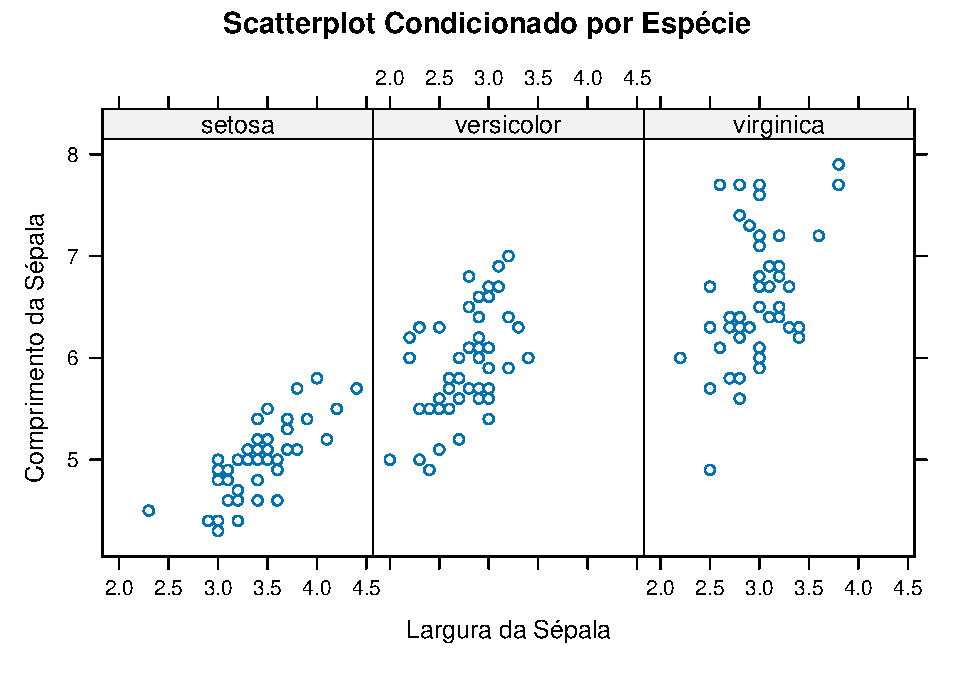
\includegraphics{_main_files/figure-latex/nome-do-chunk-1.pdf}
\caption{\label{fig:nome-do-chunk-1}Gráficos com Lattice}
\end{figure}

\begin{Shaded}
\begin{Highlighting}[]
\CommentTok{\# Histograma condicionado por uma variável}
\FunctionTok{histogram}\NormalTok{(}\SpecialCharTok{\textasciitilde{}}\NormalTok{ Petal.Length }\SpecialCharTok{|}\NormalTok{ Species, }\AttributeTok{data =}\NormalTok{ iris,}
          \AttributeTok{main =} \StringTok{"Histograma Condicionado por Espécie"}\NormalTok{,}
          \AttributeTok{xlab =} \StringTok{"Comprimento da Pétala"}\NormalTok{)}
\end{Highlighting}
\end{Shaded}

\begin{figure}
\centering
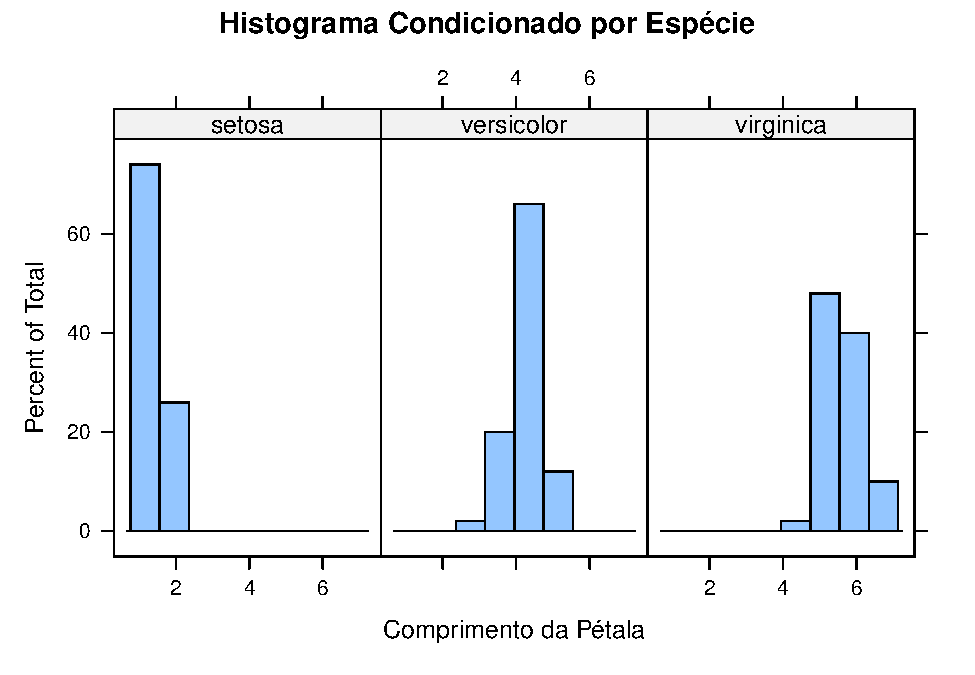
\includegraphics{_main_files/figure-latex/nome-do-chunk-2.pdf}
\caption{\label{fig:nome-do-chunk-2}Gráficos com Lattice}
\end{figure}

Acho que já deu para entender como o R funciona, né? Nos próximos capítulos, você vai aprender como trabalhar de forma eficiente no R, seguindo um fluxo de trabalho eficiente e, o melhor de tudo, reproduzível.

\hypertarget{como-trabalhar-no-r}{%
\chapter{Como trabalhar no R}\label{como-trabalhar-no-r}}

Se você já tem uma noção de R, mas ainda sente dificuldade em organizar seu fluxo de trabalho, este capítulo é para você! Utilizaremos técnicas de ciência de dados e repositórios como o GitHub para tornar o trabalho no R prazeroso e eficiente!

Iremos utilizar o banco de dados ficticios que possui erros comuns que podemos utilizar para aprender a lidar com eles sem precisar de utilizar o Excel.

Baixe a planilha fake e veja que ela possui quatro variaveis (ID, peso, numero de parasitas e local) coletadas do passarinho bem-te-vi.

\href{data/fake_data.xlsx}{Clique aqui para baixar a planilha ficticia}

Vamos importar a planilha fictícia mais para frente. Relaxe aí e finja que ela é sua.

\hypertarget{criando-um-projeto-de-r}{%
\section{Criando um projeto de R}\label{criando-um-projeto-de-r}}

Imaginemos que precisamos analisar um banco de dados de algum projeto. O primeiro passo eh criar um projeto de R, para isso voce vai no canto superior direito do RStudio (proximo a janela de environment e history) e clica:

\textbf{project (none)'' \textgreater{} new project \textgreater{} new directory \textgreater{} new project}

Ao clicar em ``New Project'', aparecerá uma janela para escolher o nome do projeto e o local no computador onde seu projeto irá ficar. Coloque o nome desejado (sugestão: ``projeto\_caranguejo''), selecione qualquer pasta no computador (sugestão: desktop) e clique em ``Criar Projeto''.

Se você fez tudo direitinho, o RStudio estará da seguinte forma. Note que ao invés de ``Project (None)'', estará o nome do projeto que você criou.

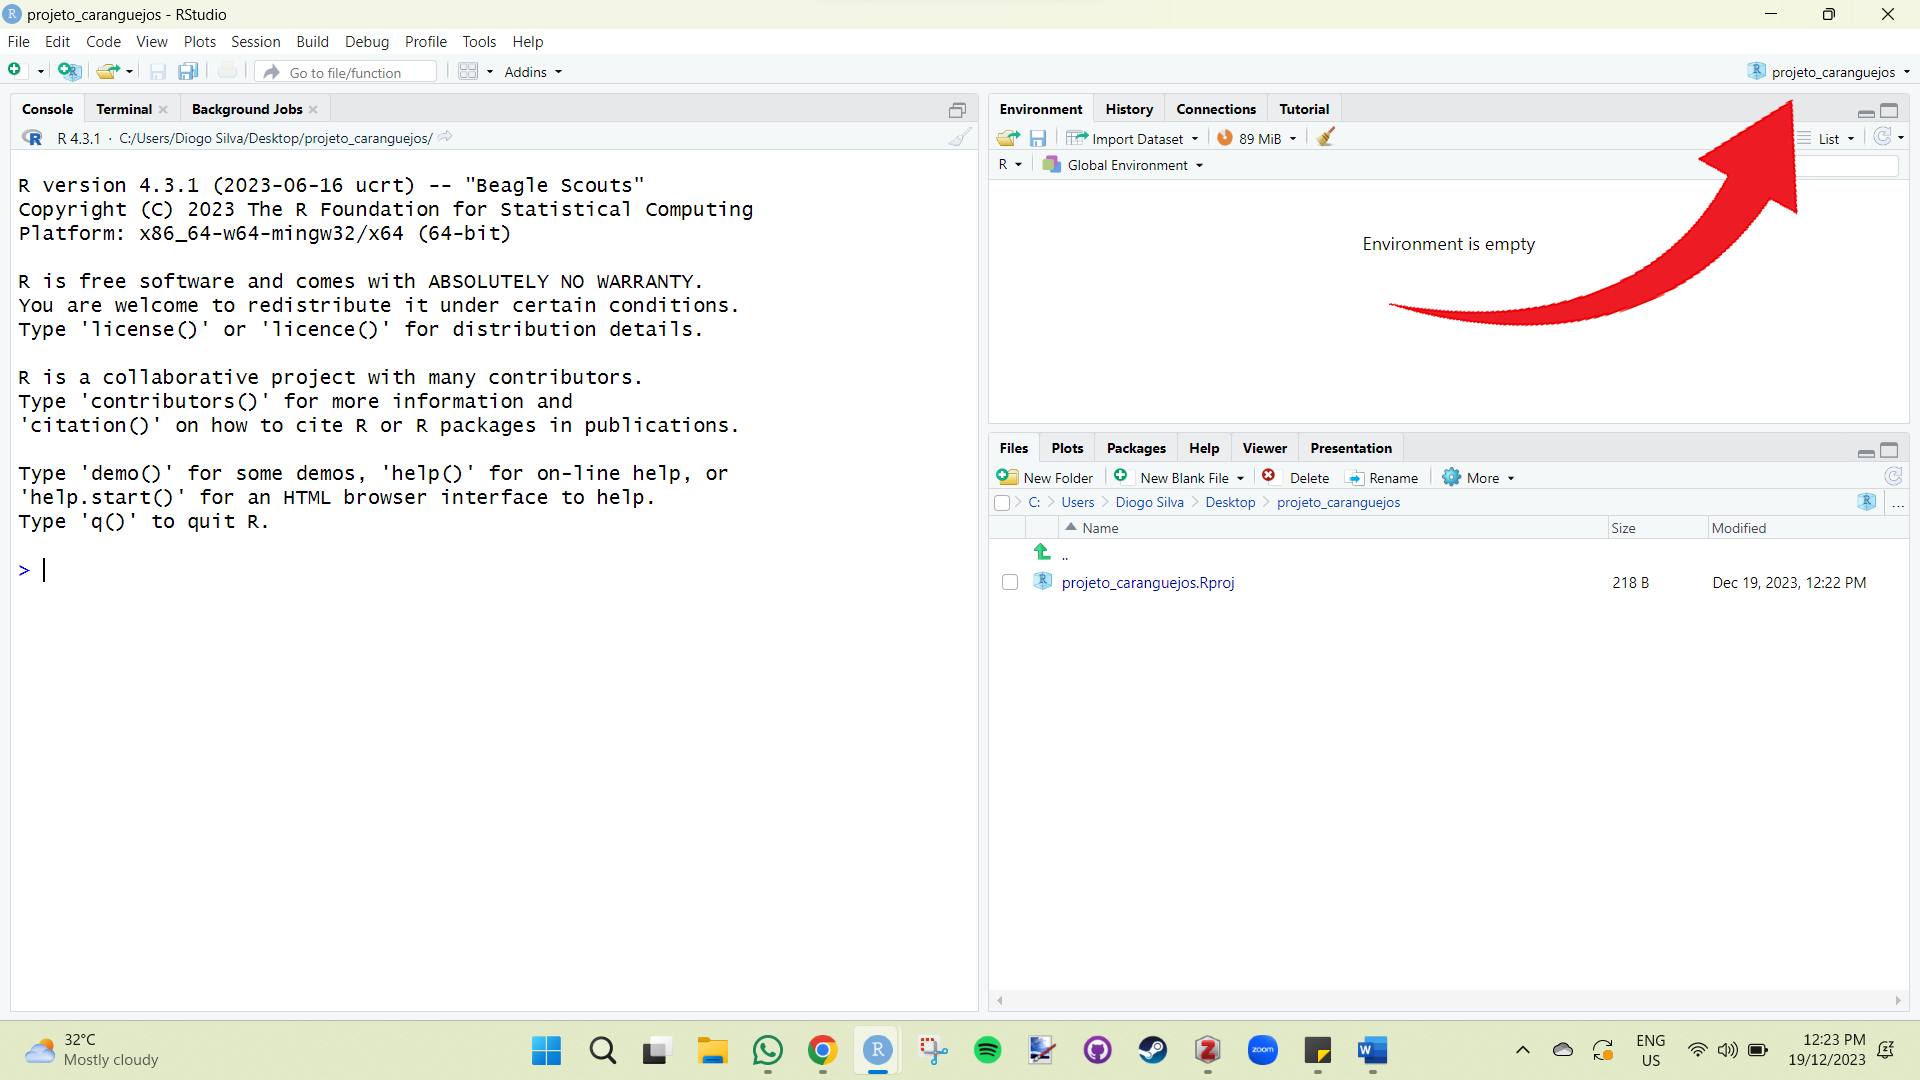
\includegraphics{img/tela_do_projeto.png}

Sugiro, meu nobre consagrado Rzeiro, que você vá no local do computador onde você criou o projeto e veja a pasta, veja o arquivo de R que foi criado. Você também pode fazer isso utilizando a janela de ``Files'', onde mostrará todas as pastas do seu diretório que, a partir de agora, será a pasta que o seu arquivo de projeto de R está situado. Todos os scripts, arquivos e planilhas que você irá utilizar nas suas análises, ficarão dentro da pasta do projeto. Isso significa que vai ficar tudo solto, bagunçado? Claro que não. Iremos criar pastas organizadas onde hospedarão cada coisa que iremos trabalhar, como por exemplo: dados brutos, dados processados, scripts, outputs, etc. Você pode criar manualmente, mas por que faríamos isso se temos o R para fazer por nós?

\hypertarget{organizando-o-projeto-de-r}{%
\section{Organizando o projeto de R}\label{organizando-o-projeto-de-r}}

Para criar as pastas de forma organizada, voce pode fazer manualmente ou utilizando o pacote ``here''.

\begin{Shaded}
\begin{Highlighting}[]
\FunctionTok{install.packages}\NormalTok{(}\StringTok{"here"}\NormalTok{)}
\FunctionTok{library}\NormalTok{(here)}
\end{Highlighting}
\end{Shaded}

Após a instalação do pacote ``here'', iremos criar uma função que criará as pastas automaticamente no nosso diretório. Não se assuste com o script da função, ela é mais simples do que parece e você não precisa entendê-lo por completo. Apenas rode o código para criar a função e depois rode o código que utiliza a função para criar as pastas.

Antes de rodar o código, certifique-se de que você está no projeto de R que você criou.

\begin{Shaded}
\begin{Highlighting}[]
\CommentTok{\# Criando funcao para criacao das pastas do projeto}
\CommentTok{\# Codigo disponibilizado pelo Gustavo Paterno (https://github.com/paternogbc)}

\NormalTok{build\_project }\OtherTok{\textless{}{-}} \ControlFlowTok{function}\NormalTok{(}\AttributeTok{type =} \StringTok{"analysis"}\NormalTok{,}
                          \AttributeTok{temp =} \ConstantTok{TRUE}\NormalTok{) \{}
  
  \ControlFlowTok{if}\NormalTok{(type }\SpecialCharTok{==} \StringTok{"analysis"}\NormalTok{)\{}
    \CommentTok{\# Data}
    \FunctionTok{dir.create}\NormalTok{(}\AttributeTok{path =}\NormalTok{ here}\SpecialCharTok{::}\FunctionTok{here}\NormalTok{(}\StringTok{"data"}\NormalTok{))}
    \FunctionTok{dir.create}\NormalTok{(}\AttributeTok{path =}\NormalTok{ here}\SpecialCharTok{::}\FunctionTok{here}\NormalTok{(}\StringTok{"data"}\NormalTok{, }\StringTok{"raw"}\NormalTok{))}
    \FunctionTok{dir.create}\NormalTok{(}\AttributeTok{path =}\NormalTok{ here}\SpecialCharTok{::}\FunctionTok{here}\NormalTok{(}\StringTok{"data"}\NormalTok{, }\StringTok{"processed"}\NormalTok{))}
    
    \CommentTok{\# outputs}
    \FunctionTok{dir.create}\NormalTok{(}\AttributeTok{path =}\NormalTok{ here}\SpecialCharTok{::}\FunctionTok{here}\NormalTok{(}\StringTok{"outputs"}\NormalTok{))}
    \FunctionTok{dir.create}\NormalTok{(}\AttributeTok{path =}\NormalTok{ here}\SpecialCharTok{::}\FunctionTok{here}\NormalTok{(}\StringTok{"outputs"}\NormalTok{, }\StringTok{"figures"}\NormalTok{))}
    \FunctionTok{dir.create}\NormalTok{(}\AttributeTok{path =}\NormalTok{ here}\SpecialCharTok{::}\FunctionTok{here}\NormalTok{(}\StringTok{"outputs"}\NormalTok{, }\StringTok{"tables"}\NormalTok{))}
    \ControlFlowTok{if}\NormalTok{(}\FunctionTok{isTRUE}\NormalTok{(temp))\{}
      \FunctionTok{dir.create}\NormalTok{(}\AttributeTok{path =}\NormalTok{ here}\SpecialCharTok{::}\FunctionTok{here}\NormalTok{(}\StringTok{"outputs"}\NormalTok{, }\StringTok{"temp"}\NormalTok{))}
\NormalTok{    \}}
    
    \CommentTok{\# scripts}
    \FunctionTok{dir.create}\NormalTok{(}\AttributeTok{path =}\NormalTok{ here}\SpecialCharTok{::}\FunctionTok{here}\NormalTok{(}\StringTok{"scripts"}\NormalTok{))}
    
    \CommentTok{\# docs}
    \CommentTok{\#dir.create(path = here::here("docs")) \#para criar a pasta docs, so tirar o comentario dessa linha}
\NormalTok{  \}}
\NormalTok{\}}

\CommentTok{\#Utilizando a funcao criada para gerar as pastas}
\FunctionTok{build\_project}\NormalTok{(}\AttributeTok{type =} \StringTok{"analysis"}\NormalTok{,}
              \AttributeTok{temp =} \ConstantTok{TRUE}\NormalTok{) }\CommentTok{\#se FALSE, nao cria a pasta temp.}
\end{Highlighting}
\end{Shaded}

Se tudo ocorreu bem, as pastas estao assim:

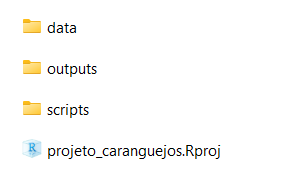
\includegraphics{img/pastas_do_projeto.png}

Dentro da pasta ``data'', você encontra as subpastas ``raw'' e ``processed''. Em ``outputs'', você encontra as subpastas ``figures'', ``temp'' e ``tables''. Em ``script'', você não encontrará nada (por enquanto). O arquivo com o símbolo do R ``projeto\_caranguejos.Rproj'' é o seu projeto de R. Você pode abri-lo (dando duplo clique) toda vez que você for trabalhar no projeto. Isso abrirá o RStudio já com o seu projeto aberto e pronto para trabalhar.

\begin{itemize}
\tightlist
\item
  Feche o RStudio e abra-o novamente dando clique duplo no seu projeto de R.
\end{itemize}

Agora você tem tudo pronto para começar a trabalhar com um fluxo de trabalho eficiente e reprodutível!

\hypertarget{trabalhando-em-um-projeto-de-r}{%
\section{Trabalhando em um projeto de R}\label{trabalhando-em-um-projeto-de-r}}

Antes de tudo baixe a planilha de dados ficticios (caso nao tenha baixado ainda) de uma especie de passarinho (tambem ficticia), que contem informacoes ficticias sobre peso (g) e quantidade de parasitas de tres diferentes localidades do bem-te-vi:

\href{data/fake_data.xlsx}{Clique aqui para baixar a planilha ficticia}

Na pasta \textbf{data \textgreater{} raw}, você adiciona sua planilha de dados brutos fictícia (fake\_data.xlsx). O fluxo de trabalho será o mais simples possível, mas envolverá etapas essenciais da análise de dados.

\textbf{Limpar dados brutos \textgreater{} Realizar análise \textgreater{} Mostrar gráficos}

Para limpar a planilha de dados brutos, iremos criar um script para isso. Utilizaremos funções do pacote \emph{dplyr} para modificar nomes das variáveis, nomes dos fatores, analisar dados faltantes, entre outras coisas.

\hypertarget{etapa-1-limpar-dados}{%
\subsection{Etapa 1: limpar dados}\label{etapa-1-limpar-dados}}

Vamos criar um script para limpar nossos dados brutos. Monte o script completo utilizando os codigos que irei fornecendo a seguir copiando e colando no seu RStudio. Assim, a primeira coisa que iremos fazer do script eh seu cabecalho. Utilizaremos os comentarios para criar um cabecalho com as informacoes de titulo, autores e data.

\begin{Shaded}
\begin{Highlighting}[]

\CommentTok{\# Script to load and clean raw data flores iris}
\CommentTok{\# Author: Marilia T. Ericcson}
\CommentTok{\# Data: 2019{-}11{-}06}
\end{Highlighting}
\end{Shaded}

Após isso, utilizaremos os comentários para organizar o script em tópicos, fazendo isso manualmente ou utilizando o atalho: \textbf{Ctrl + Shift + R}. A primeira parte do código é a instalação dos pacotes que iremos utilizar no processo.

\begin{Shaded}
\begin{Highlighting}[]

\CommentTok{\# Packages {-}{-}{-}{-}{-}{-}{-}{-}{-}{-}{-}{-}{-}{-}{-}{-}{-}{-}{-}{-}{-}{-}{-}{-}{-}{-}{-}{-}{-}{-}{-}{-}{-}{-}{-}{-}{-}{-}{-}{-}{-}{-}{-}{-}{-}{-}{-}{-}{-}{-}{-}{-}{-}{-}{-}{-}{-}{-}{-}{-}{-}}
\CommentTok{\# Caso nao tenha os pacotes instalados, instale!}

\FunctionTok{library}\NormalTok{(dplyr)  }\CommentTok{\#Pacote com funcoes para manipular dados}
\FunctionTok{library}\NormalTok{(readxl) }\CommentTok{\#Pacote com funcao para importar planilha em formato de excel (xlsx)}
\end{Highlighting}
\end{Shaded}

Segundo, importamos o banco de dados a ser processado (limpado) utilizando a função \emph{read.csv()} e atribuindo (\textless-) a um objeto que iremos chamar de ``dados''. Para importar, você só precisa especificar o caminho do diretório em que o arquivo está inserido. Como estamos utilizando o projeto de R, o diretório é onde o projeto está. Dessa forma, não há necessidade de dizer para o R qual é o seu diretório de trabalho. Logo, fica fácil importar os dados brutos pois sabemos que ele está na pasta ``dados \textgreater{} raw \textgreater{} iris.csv''. Dizemos isso para o R utilizando os nomes das pastas separados por barras e, por fim, o nome do arquivo (iris) e sua extensão (.csv).

\begin{Shaded}
\begin{Highlighting}[]

\CommentTok{\# Load data {-}{-}{-}{-}{-}{-}{-}{-}{-}{-}{-}{-}{-}{-}{-}{-}{-}{-}{-}{-}{-}{-}{-}{-}{-}{-}{-}{-}{-}{-}{-}{-}{-}{-}{-}{-}{-}{-}{-}{-}{-}{-}{-}{-}{-}{-}{-}{-}{-}{-}{-}{-}{-}{-}{-}{-}{-}{-}{-}{-}{-}{-}{-}}
\NormalTok{dados }\OtherTok{\textless{}{-}} \FunctionTok{read\_excel}\NormalTok{(}\StringTok{"data/raw/fake\_data.xlsx"}\NormalTok{)}
\end{Highlighting}
\end{Shaded}

Agora que o banco de dados foi importado, podemos fazer um check up basico utilizando algumas funcoes. Como assim check up basico? Ver o numero de observacoes, se tem dado faltando ou observacao duplicada, essas coisas.

\begin{Shaded}
\begin{Highlighting}[]

\CommentTok{\# 1. Check up basico {-}{-}{-}{-}{-}{-}{-}{-}{-}{-}{-}{-}{-}{-}{-}{-}{-}{-}{-}{-}{-}{-}{-}{-}{-}{-}{-}{-}{-}{-}{-}{-}{-}{-}{-}{-}{-}{-}{-}{-}{-}{-}{-}{-}{-}{-}{-}{-}{-}{-}{-}{-}{-}{-}{-}{-}{-}{-}{-}{-}{-}{-}}
\FunctionTok{nrow}\NormalTok{(dados)             }\CommentTok{\# Quantas linhas (observacoes) tem no banco de dados?}
\FunctionTok{str}\NormalTok{(dados)              }\CommentTok{\# quais as classes das variaveis?}
\FunctionTok{attributes}\NormalTok{(dados)       }\CommentTok{\# quais atributos?}
\FunctionTok{head}\NormalTok{(dados)             }\CommentTok{\# Primeiras linhas do banco de dados.}
\FunctionTok{any}\NormalTok{(}\FunctionTok{duplicated}\NormalTok{(dados))  }\CommentTok{\# Checar se tem linhas duplicadas.}
\FunctionTok{any}\NormalTok{(}\FunctionTok{is.na}\NormalTok{(dados))       }\CommentTok{\# Checar se tem dado faltando (NA).}
\end{Highlighting}
\end{Shaded}

Às vezes, os nomes das variáveis não são fáceis de trabalhar, possuindo espaços, acentos, letras maiúsculas e minúsculas, e nomes confusos. Além de complicar o código, o nome de algumas variáveis pode bugá-lo (caso das acentuações de palavras em português). Então, vamos mudar o nome das variáveis utilizando a função \emph{rename()} do pacote \textbf{dplyr}. Iremos deixar os nomes mais fáceis de trabalhar, deixando todas as letras minúsculas.

\begin{Shaded}
\begin{Highlighting}[]

\CommentTok{\# 3. Renomeando o nome das variaveis {-}{-}{-}{-}{-}{-}{-}{-}{-}{-}{-}{-}{-}{-}{-}{-}{-}{-}{-}{-}{-}{-}{-}{-}{-}{-}{-}{-}{-}{-}{-}{-}{-}{-}{-}{-}{-}{-}{-}{-}{-}{-}{-}{-}{-}{-}{-}{-}{-}{-}{-}{-}{-}{-}{-}}
\CommentTok{\#ver nome das colunas (variaveis) {-}{-}{-}{-}}
\FunctionTok{colnames}\NormalTok{(dados)}

\CommentTok{\#Renomeando variaveis {-}{-}{-}{-}}
\CommentTok{\#Vamos renomear de forma a tirar espacos e manter apenas letras minusculas.}
\NormalTok{dados\_renamed }\OtherTok{\textless{}{-}} \FunctionTok{rename}\NormalTok{(dados,           }
                        \AttributeTok{id =}\NormalTok{ ID,  }\CommentTok{\#nomes das variaveis (nome novo = nome antigo)}
                        \AttributeTok{peso\_g  =} \StringTok{\textasciigrave{}}\AttributeTok{Peso (g)}\StringTok{\textasciigrave{}}\NormalTok{,}
                        \AttributeTok{total\_parasitas =} \StringTok{\textasciigrave{}}\AttributeTok{Total de parasitas}\StringTok{\textasciigrave{}}\NormalTok{,}
                        \AttributeTok{local  =}\NormalTok{ Local}
\NormalTok{                        )}
\FunctionTok{colnames}\NormalTok{(dados\_renamed)}
\end{Highlighting}
\end{Shaded}

Note que quando existe espaço, o nome da variável precisa estar entre crases.
Agora vamos dizer para o R os tipos de nossas variáveis. Um problema muito comum é o R não reconhecer que a variável categórica não possui fatores, mesmo possuindo. Por exemplo, em ``iris'', temos a variável categórica `Species' com seus fatores (setosa, versicolor, virginica). É possível que no seu banco de dados, o R não reconheça isso, então vamos utilizar a função \emph{levels()} para verificar se o R entendeu quais são os fatores. Se o R retornar NULL, você precisa dizer para o R utilizando a função \emph{as.factor()}.

\begin{Shaded}
\begin{Highlighting}[]

\CommentTok{\# 4. Consertar fatores  {-}{-}{-}{-}{-}{-}{-}{-}{-}{-}{-}{-}{-}{-}{-}{-}{-}{-}{-}{-}{-}{-}{-}{-}{-}{-}{-}{-}{-}{-}{-}{-}{-}{-}{-}{-}{-}{-}{-}{-}{-}{-}{-}{-}{-}{-}{-}{-}{-}{-}{-}{-}{-}{-}{-}{-}}
\CommentTok{\# ver quais fatores estao na variavel local}
\FunctionTok{levels}\NormalTok{(dados\_renamed}\SpecialCharTok{$}\NormalTok{local) }\CommentTok{\#Se retornar NULL eh porque nao ta reconhecendo como fator.}

\CommentTok{\# Transformando em fator {-}{-}{-}{-}}
\NormalTok{dados\_renamed}\SpecialCharTok{$}\NormalTok{local }\OtherTok{\textless{}{-}} \FunctionTok{as.factor}\NormalTok{(dados\_renamed}\SpecialCharTok{$}\NormalTok{local)}

\CommentTok{\# checar fatores}
\FunctionTok{levels}\NormalTok{(dados\_renamed}\SpecialCharTok{$}\NormalTok{local)}
\end{Highlighting}
\end{Shaded}

Agora podemos renomear o nome dos fatores de uma variável categórica utilizando a função \emph{recode\_factor()}. Nesse processo, podemos identificar erros de digitação que ocorreram durante o planilhamento dos dados. Por exemplo, você pode ter digitado ``Macho'', ``macho'' e ``male'' na variável sexo durante o planilhamento. O R vai identificar os três como sendo fatores diferentes, mas na verdade são o mesmo fator. Portanto, é necessário que seja padronizado.

\begin{Shaded}
\begin{Highlighting}[]
\CommentTok{\# 4.1 Renomear fatores}

\CommentTok{\#Checar fatores}
\FunctionTok{levels}\NormalTok{(dados\_renamed}\SpecialCharTok{$}\NormalTok{local)}
\end{Highlighting}
\end{Shaded}

Veja que aqui deveríamos ter apenas três fatores: floresta, urbano e parque. Mas, devido a erros de digitação, o R entende que são fatores diferentes. Isso é muito comum em planilhas de dados grandes, e você teria que fazer isso manualmente, identificando cada erro. Imagina o trabalhão.

\begin{Shaded}
\begin{Highlighting}[]
\CommentTok{\#Renomear fatores}
\NormalTok{dados\_renamed}\SpecialCharTok{$}\NormalTok{local }\OtherTok{\textless{}{-}} \FunctionTok{recode\_factor}\NormalTok{(dados\_renamed}\SpecialCharTok{$}\NormalTok{local,   }\CommentTok{\#variavel categorica}
                                     \AttributeTok{Floresta =} \StringTok{"floresta"}\NormalTok{,         }\CommentTok{\#mudando nome Floresta para floresta}
                                     \AttributeTok{park =} \StringTok{"parque"}\NormalTok{,}
                                     \AttributeTok{parque. =} \StringTok{"parque"}\NormalTok{,}
                                     \AttributeTok{urban =} \StringTok{"urbano"}\NormalTok{,}
                                     \AttributeTok{Urbano =} \StringTok{"urbano"}\NormalTok{)}

\CommentTok{\#check factors}
\FunctionTok{levels}\NormalTok{(dados\_renamed}\SpecialCharTok{$}\NormalTok{local)}
\end{Highlighting}
\end{Shaded}

Agora sim! Temos os três fatores bonitinhos. Agora que limpamos nossos dados brutos, iremos exportar nossa planilha limpa. Perceba que o processo do script é colocar a planilha bruta de um lado e sair limpa e bonitinha do outro. É com os dados processados que iremos trabalhar de fato. Vamos salvar sempre no formato CSV, por ser um formato mais simples, leve e estável.

\begin{Shaded}
\begin{Highlighting}[]
\CommentTok{\# 8. Salvar dado processado {-}{-}{-}{-}{-}{-}{-}{-}{-}{-}{-}{-}{-}{-}{-}{-}{-}{-}{-}{-}{-}{-}{-}{-}{-}{-}{-}{-}{-}{-}{-}{-}{-}{-}{-}{-}{-}{-}{-}{-}{-}{-}{-}{-}{-}{-}{-}{-}{-}{-}{-}{-}}
\FunctionTok{write.csv}\NormalTok{(}\AttributeTok{x =}\NormalTok{ dados\_renamed,    }\CommentTok{\#nome da planilha que voce quer exportar}
          \AttributeTok{file =} \StringTok{"data/processed/processed\_fake\_data.csv"}\NormalTok{, }\CommentTok{\#local e nome da planilha exportada}
          \AttributeTok{row.names =} \ConstantTok{FALSE}\NormalTok{)  }\CommentTok{\#sempre utilizaremos row.names = FALSE}
\end{Highlighting}
\end{Shaded}

O processo de manipulação de dados no R é bastante completo, e existem diferentes formas de limpar seus dados brutos. O pacote \textbf{dplyr} possui funções capazes de selecionar variáveis, selecionar linhas, criar variáveis, criar subconjuntos, entre outras. Para aprimorar seu script de limpeza de dados, você precisará aprender sobre manipulação de dados e incluir no processo os códigos no seu script. Por sorte, existe muito material disponível na internet sobre o assunto. Talvez algum dia eu crie um material sobre manipulação de dados com dplyr, mas aqui esse não é meu objetivo. Meu objetivo é simplesmente fornecer o esqueleto teórico, dando base para crescer de forma mais direcionada.

Por fim, não esqueça de salvar o script na pasta script com o nome `01\_clean\_raw\_data'.

\hypertarget{etapa-2-fazer-analise}{%
\subsection{Etapa 2: fazer analise}\label{etapa-2-fazer-analise}}

Com a planilha bruta processada, podemos realizar testes estatísticos em um novo script para responder à nossa hipótese. Vamos supor que nossa pergunta seja saber se existe diferença na infestação de parasitas em cada local. Organizaremos o script de análise de forma semelhante ao script de limpeza, ou seja, escreveremos um cabeçalho, carregaremos pacotes, importaremos e analisaremos dados de forma organizada.

Vamos fazer um cabeçalho para nosso script de análise.

\begin{Shaded}
\begin{Highlighting}[]

\CommentTok{\# Script para analisar dados}
\CommentTok{\# Author: seu nome}
\CommentTok{\# Data: 2019{-}11{-}07}
\end{Highlighting}
\end{Shaded}

Vamos criar o código para carregar os pacotes que iremos utilizar.

\begin{Shaded}
\begin{Highlighting}[]

\CommentTok{\#Carregar pacotes}
\FunctionTok{library}\NormalTok{(broom)}
\end{Highlighting}
\end{Shaded}

Dessa vez, iremos importar a planilha limpa e processada. Note que o caminho de importação é similar ao caminho que exportamos no script de limpeza.

\begin{Shaded}
\begin{Highlighting}[]

\CommentTok{\# Load data {-}{-}{-}{-}{-}{-}{-}{-}{-}{-}{-}{-}{-}{-}{-}{-}{-}{-}{-}{-}{-}{-}{-}{-}{-}{-}{-}{-}{-}{-}{-}{-}{-}{-}{-}{-}{-}{-}{-}{-}{-}{-}{-}{-}{-}{-}{-}{-}{-}{-}{-}{-}{-}{-}{-}{-}{-}{-}{-}{-}{-}{-}{-}}
\NormalTok{dados }\OtherTok{\textless{}{-}} \FunctionTok{read.csv}\NormalTok{(}\StringTok{"data/processed/processed\_iris.csv"}\NormalTok{)}
\end{Highlighting}
\end{Shaded}

Vamos fazer um check basico.

\begin{Shaded}
\begin{Highlighting}[]

\CommentTok{\# 1. Check up basico {-}{-}{-}{-}{-}{-}{-}{-}{-}{-}{-}{-}{-}{-}{-}{-}{-}{-}{-}{-}{-}{-}{-}{-}{-}{-}{-}{-}{-}{-}{-}{-}{-}{-}{-}{-}{-}{-}{-}{-}{-}{-}{-}{-}{-}{-}{-}{-}{-}{-}{-}{-}{-}{-}{-}{-}{-}{-}{-}{-}{-}{-}}
\FunctionTok{head}\NormalTok{(dados)}
\FunctionTok{str}\NormalTok{(dados)}
\FunctionTok{leves}\NormalTok{(dados}\SpecialCharTok{$}\NormalTok{local)}
\end{Highlighting}
\end{Shaded}

Vamos realizar uma análise para ver se existe diferença na quantidade de parasitas encontrada nos bem-te-vis de cada local. Para isso, iremos utilizar o teste não paramétrico de Kruskal-Wallis através da função kruskal.test(). Nessa função, você precisa dizer qual sua variável numérica de interesse em relação a (\textasciitilde) sua variável categórica e seus grupos (fatores). Veja que o p-value é menor que 0.05, então dizemos que existe diferença da largura entre as três espécies.

\begin{Shaded}
\begin{Highlighting}[]

\CommentTok{\#realizando o teste}
\NormalTok{kw }\OtherTok{\textless{}{-}} \FunctionTok{kruskal.test}\NormalTok{(dados}\SpecialCharTok{$}\NormalTok{total\_parasitas }\SpecialCharTok{\textasciitilde{}}\NormalTok{ dados}\SpecialCharTok{$}\NormalTok{local)}
\NormalTok{kw}
\end{Highlighting}
\end{Shaded}

Vamos salvar o resultado em uma tabela organizada (tidy) utilizando a função \emph{tidy()} do pacote \textbf{broom}.

\begin{Shaded}
\begin{Highlighting}[]

\CommentTok{\#Convertendo tabela para formato tidy}
\NormalTok{table\_kw }\OtherTok{\textless{}{-}} \FunctionTok{tidy}\NormalTok{(kw\_test)}
\NormalTok{table\_kw}
\end{Highlighting}
\end{Shaded}

Agora salvaremos essa tabela na nossa pasta outputs em tables.

\begin{Shaded}
\begin{Highlighting}[]

\CommentTok{\#Exportando resultado}
\FunctionTok{write.csv}\NormalTok{(}\AttributeTok{x =}\NormalTok{ table\_kw,                                 }
          \AttributeTok{file =} \StringTok{"outputs/tables/resultado\_kw.csv"}\NormalTok{,}
          \AttributeTok{row.names =} \ConstantTok{FALSE}\NormalTok{)}
\end{Highlighting}
\end{Shaded}

Maravilha! Já temos nosso segundo script pronto. Agora é só salvá-lo na pasta script com o nome `02\_kruskal\_test'.

\hypertarget{etapa-3-criar-grafico}{%
\subsection{Etapa 3: criar grafico}\label{etapa-3-criar-grafico}}

Agora vamos criar o gráfico para representar nosso resultado de que existe diferença na largura das pétalas entre as espécies de iris.

\begin{Shaded}
\begin{Highlighting}[]
 
\CommentTok{\# Script para criar graficos}
\CommentTok{\# Author: seu nome}
\CommentTok{\# Data: 2019{-}11{-}07}
 
\CommentTok{\#Carregar pacotes}
\FunctionTok{library}\NormalTok{(ggplot2)}

\CommentTok{\# Load data {-}{-}{-}{-}{-}{-}{-}{-}{-}{-}{-}{-}{-}{-}{-}{-}{-}{-}{-}{-}{-}{-}{-}{-}{-}{-}{-}{-}{-}{-}{-}{-}{-}{-}{-}{-}{-}{-}{-}{-}{-}{-}{-}{-}{-}{-}{-}{-}{-}{-}{-}{-}{-}{-}{-}{-}{-}{-}{-}{-}{-}{-}{-}}
\NormalTok{dados }\OtherTok{\textless{}{-}} \FunctionTok{read.csv}\NormalTok{(}\StringTok{"data/processed/processed\_fake\_data.csv"}\NormalTok{)}

\CommentTok{\# 1. Basic checks {-}{-}{-}{-}{-}{-}{-}{-}{-}{-}{-}{-}{-}{-}{-}{-}{-}{-}{-}{-}{-}{-}{-}{-}{-}{-}{-}{-}{-}{-}{-}{-}{-}{-}{-}{-}{-}{-}{-}{-}{-}{-}{-}{-}{-}{-}{-}{-}{-}{-}{-}{-}{-}{-}{-}{-}{-}{-}{-}{-}{-}{-}}
\FunctionTok{head}\NormalTok{(dados)}
\FunctionTok{str}\NormalTok{(dados)}
\FunctionTok{leves}\NormalTok{(dados}\SpecialCharTok{$}\NormalTok{species)}

\CommentTok{\# 2. Criar grafico boxplot {-}{-}{-}{-}{-}{-}{-}{-}{-}{-}{-}{-}{-}{-}{-}{-}{-}{-}{-}{-}{-}{-}{-}{-}{-}{-}{-}{-}{-}{-}{-}{-}{-}{-}{-}{-}{-}{-}{-}{-}{-}{-}{-}{-}{-}{-}{-}{-}{-}{-}{-}{-}{-}}

\NormalTok{grafico }\OtherTok{\textless{}{-}} \FunctionTok{ggplot}\NormalTok{(dados, }\FunctionTok{aes}\NormalTok{(}\AttributeTok{x =}\NormalTok{ species, }\AttributeTok{y =}\NormalTok{ petal\_width))}\SpecialCharTok{+}
  \FunctionTok{geom\_boxplot}\NormalTok{()}

\NormalTok{grafico}

\CommentTok{\# 3. Salvando grafico {-}{-}{-}{-}{-}{-}{-}{-}{-}{-}{-}{-}{-}{-}{-}{-}{-}{-}{-}{-}{-}{-}{-}{-}{-}{-}{-}{-}{-}{-}{-}{-}{-}{-}{-}{-}{-}{-}{-}{-}{-}{-}{-}{-}{-}{-}{-}{-}{-}{-}{-}{-}{-}{-}{-}{-}{-}{-}}

\FunctionTok{ggsave}\NormalTok{(}\AttributeTok{plot =}\NormalTok{ grafico,    }\CommentTok{\#nome do grafico}
       \AttributeTok{filename =} \StringTok{"output/figures/Grafico\_boxplot.png"}\NormalTok{, }\CommentTok{\#nome do grafico exportado}
       \AttributeTok{width =} \DecValTok{10}\NormalTok{,                             }\CommentTok{\#largura do grafico}
       \AttributeTok{height =} \DecValTok{10}\NormalTok{,                            }\CommentTok{\#Altura do grafico}
       \AttributeTok{dpi =} \DecValTok{300}\NormalTok{)                              }\CommentTok{\#resolucao do grafico}
\end{Highlighting}
\end{Shaded}

\begin{figure}
\centering
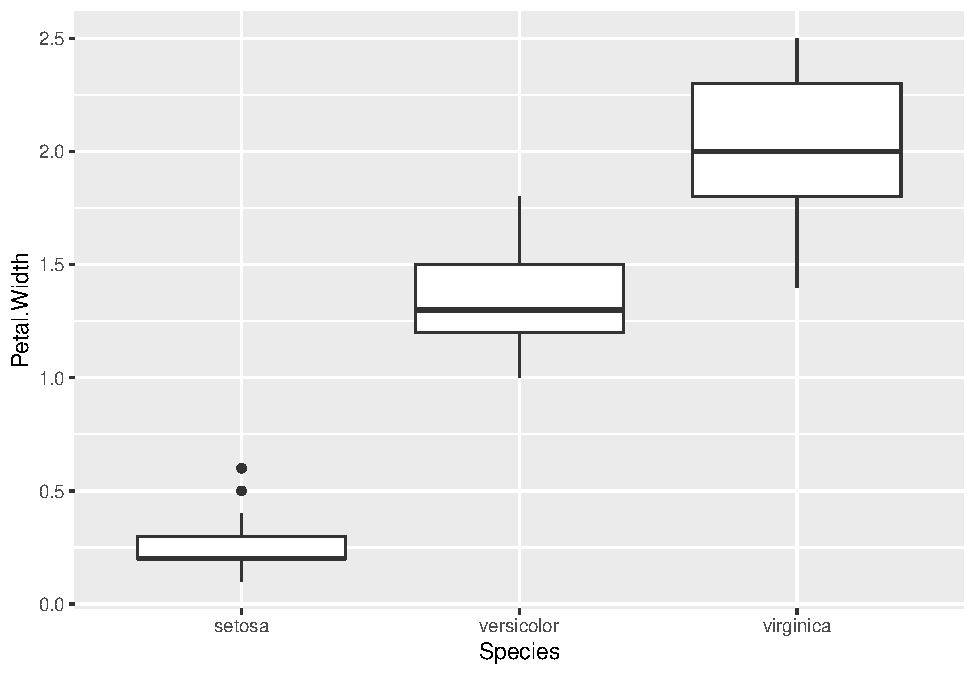
\includegraphics{_main_files/figure-latex/graph-1.pdf}
\caption{\label{fig:graph}ggplot2}
\end{figure}

Você acabou de criar um gráfico utilizando o pacote ggplot2, que é o pacote mais utilizado para produção de gráficos no R. O código pode parecer um pouco confuso no início, mas não precisa estudar muito para perceber que ele é muito simples e intuitivo. Para aprender mais sobre gráficos, sugiro os livros: \href{https://rkabacoff.github.io/datavis/}{Data Visualization: A practical introduction} e \href{https://r-graphics.org/}{R Graphics Cookbook}.

Não esqueça de salvar o script com o nome `03\_grafico'.

\hypertarget{etapa-4-replicabilidade}{%
\subsection{Etapa 4: Replicabilidade}\label{etapa-4-replicabilidade}}

O seu projeto está organizado de forma que se torna fácil a replicabilidade em qualquer computador, gerando todos seus outputs (tabelas e figuras) automaticamente! Para isso, você precisa manter e \textbf{JAMAIS deletar} ou modificar seus dados brutos (pasta raw). Todos os demais arquivos podem ser produzidos com um clique a partir dos seus dados brutos, portanto, podem ser deletados. Isso se torna útil ao compartilhar seus dados com alguém, em que você pode zipar todo seu projeto, enviar para um contribuidor, e ele poderá ter acesso a tudo rodando apenas um script. É esse script que iremos fazer agora.

\begin{Shaded}
\begin{Highlighting}[]
\CommentTok{\# Script to run all project code}
\CommentTok{\# Importante: reinicie o R antes de rodar esse script session \textgreater{} restart R}

\CommentTok{\# Start{-}{-}{-}{-}}
\CommentTok{\# 1. Run all scripts again on a fresh R section{-}{-}{-}{-}{-}{-}{-}{-}{-}{-}{-}{-}{-}{-}{-}{-}{-}{-}{-}{-}{-}{-}{-}{-}{-}{-}{-}{-}{-}{-}{-}{-}{-}}
\CommentTok{\# 1.1 Load and clean data{-}{-}{-}{-}}
\FunctionTok{source}\NormalTok{(}\AttributeTok{file =} \StringTok{"script/01\_clean\_raw\_data.R"}\NormalTok{)}

\CommentTok{\# 1.2 Run analysis {-}{-}{-}{-}{-}{-}{-}{-}{-}{-}{-}{-}{-}{-}{-}{-}{-}{-}{-}{-}{-}{-}{-}{-}{-}{-}{-}{-}{-}{-}{-}{-}{-}{-}{-}{-}{-}{-}{-}{-}{-}{-}{-}{-}{-}{-}{-}{-}{-}{-}{-}{-}{-}{-}{-}{-}{-}{-}{-}{-}{-}}
\FunctionTok{source}\NormalTok{(}\AttributeTok{file =} \StringTok{"script/02\_kruskal\_test.R"}\NormalTok{)}

\CommentTok{\# 1.3 Plot figures{-}{-}{-}{-}{-}{-}{-}{-}{-}{-}{-}{-}{-}{-}{-}{-}{-}{-}{-}{-}{-}{-}{-}{-}{-}{-}{-}{-}{-}{-}{-}{-}{-}{-}{-}{-}{-}{-}{-}{-}{-}{-}{-}{-}{-}{-}{-}{-}{-}{-}{-}{-}{-}{-}{-}{-}{-}{-}{-}{-}{-}{-}}
\FunctionTok{source}\NormalTok{(}\AttributeTok{file =} \StringTok{"script/03\_grafico.R"}\NormalTok{)}
\end{Highlighting}
\end{Shaded}

Ao rodar este código, todos os seus scripts são executados, e todos os seus outputs e planilhas processadas são gerados. Mas lembre-se, seu dado bruto contido na pasta data/raw não pode ser deletado ou modificado.

Salve este script com o nome ``run\_project''.

\hypertarget{git-e-github}{%
\chapter{Git e GitHub}\label{git-e-github}}

\hypertarget{criando-funcoes-avancadas}{%
\chapter{Criando funcoes avancadas}\label{criando-funcoes-avancadas}}

\hypertarget{criando-pacotes}{%
\chapter{Criando pacotes}\label{criando-pacotes}}

  \bibliography{book.bib}

\end{document}
